\title{Statistics and Data Analytics}
\author{Guanqun Cao\\
\texttt{guanqun.cao@tut.fi}}
\date{\today}
\documentclass[10pt, a4paper]{article}
\usepackage{graphicx,amssymb,amstext,amsmath}
\usepackage{color}
\usepackage{xcolor}
\usepackage{bm}
\usepackage{hyperref}
\usepackage{amsmath}
\usepackage{setspace}
\usepackage{fancyhdr}
\usepackage{fullpage}
\newif\ifarial
\usepackage{pslatex} % Times New Roman
\hypersetup{colorlinks=true, linkcolor=blue!50!black}
\begin{document}
\graphicspath{{/home/cao/Dropbox/thesis/Documents/Notes/statistics/figures/}}
\maketitle
\pagestyle{plain}
\tableofcontents
\section{Theory}
\subsection{Basics}
Statistics is all about is converting data into useful information.\\
The process of drawing a statistics:
\begin{enumerate}
\item The process of statistics starts when we identify what group we want to study or learn something about. We call this group the \emph{population}. 
\item We cannot study the entire population and therefore, a more practical approach would be to examine and collect data only from a subgroup of the population, which we call a \emph{sample}. 
\item We need to summarize the list in meaningful way, which is \emph{exploratory data analysis}.
\item Before we can do so, we need to look at how the sample we're using may differ from the population as a whole, so that we can factor that into our analysis. To examine this difference, we use \emph{probability}. 
\item Finally, we can use what we've discovered about our sample to draw conclusions about our population. We call this final step in the process \emph{inference}.
\end{enumerate}
In other words, there is a four-step process that encompasses statistics: data production, exploratory data analysis, probability, and inference.\\
\begin{figure}
    [h!]
    \centering
    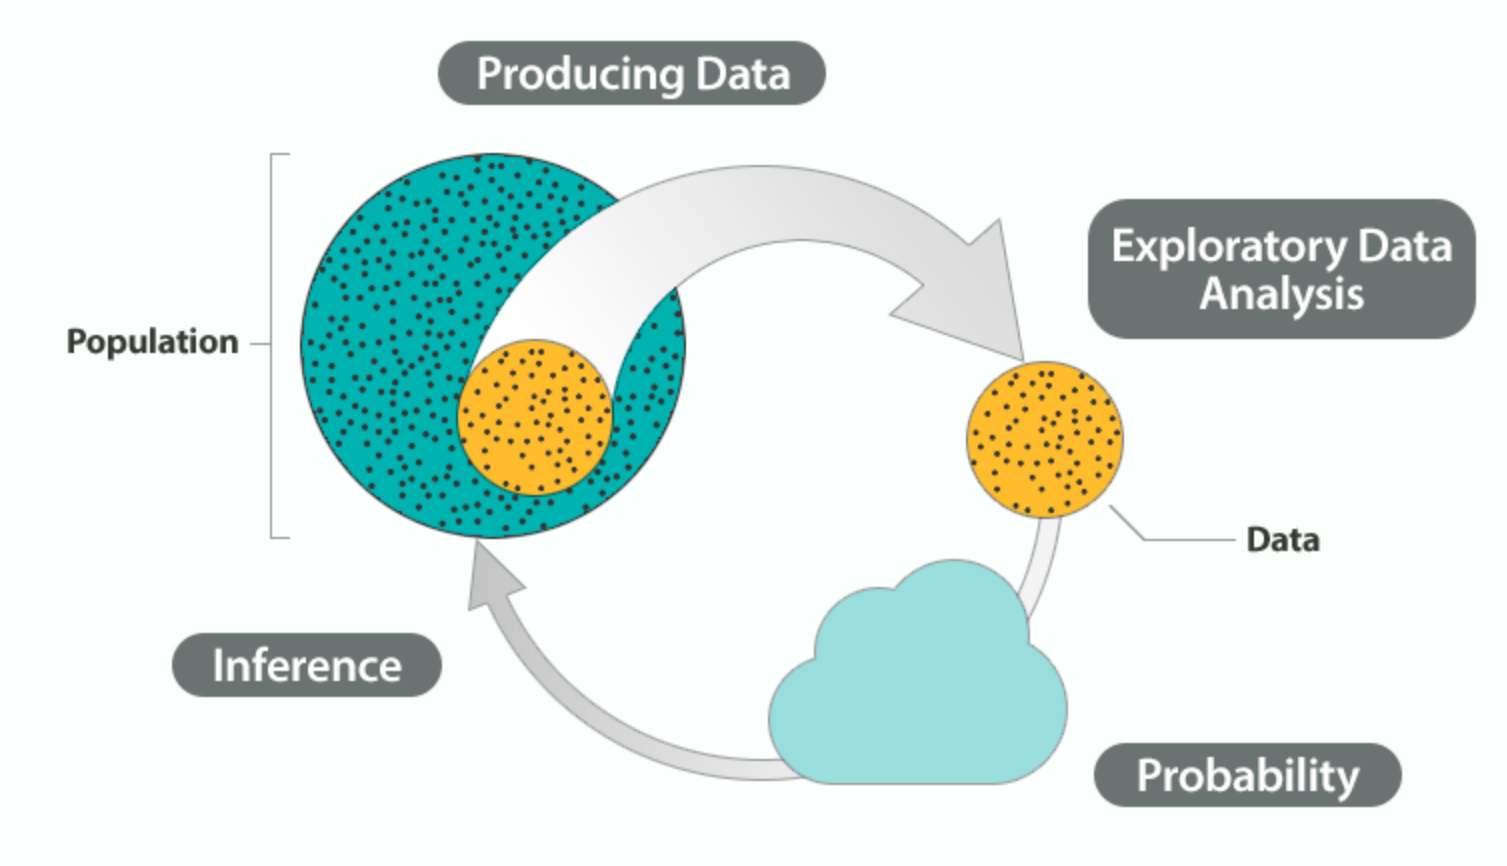
\includegraphics[width=.6\textwidth]{bigpic.png}
    \caption{An illustration of big picture of statistics.}
\end{figure}
Terminology:
\begin{itemize}
\item
\emph{Data} are pieces of information about individuals organized into variables. By an individual, we mean a particular person or object. 
\item By a \emph{variable}, we mean a particular characteristic of the individual.
\item A \emph{dataset} is a set of data identified with particular circumstances. Datasets are typically displayed in tables, in which rows represent individuals and columns represent variables.
\item Categorical variables take category or label values and place an individual into one of several groups. Each observation can be placed in only one category, and the categories are mutually exclusive.
\item Quantitative variables take numerical values and represent some kind of measurement.
\end{itemize}
Scales of Measurement / Types of Variable
\begin{itemize}
\item From least to most precise: Norminal, ordinal, interval and ratio. 
\item The nominal scale of measurement is a qualitative measure that uses discrete categories to describe a characteristic of the research participants.
\item An ordinal scale of measurement rank-orders participants on some scale or attribute, but the difference between numbers does not convey fixed or equal differences.
\item 
  The interval scale of measurement takes numerical form, and the distance between pairs of consecutive numbers is assumed to be equal. However, interval variables do not have a meaningful zero point; thus, a zero does not mean the absence of the attribute, but rather it is a particular (but arbitrary) point on the scale.
\item 
The ratio scale of measurement is similar to the interval scale. The main difference between interval and ratio measurements has to do with how we interpret a value of zero. For ratio measures, the zero is meaningful and tell us that the attribute is not present in the participant. 
\end{itemize}
The \emph{distribution} of a variable suggests: what values the variable takes, and
how often the variable takes those values.\\[1mm]
\subsection{Graphical illustration}
Pictograms
\begin{itemize}
\item The distribution of a categorical variable is summarized using:
\item Graphical display: pie chart or bar chart, supplemented by
\item Numerical summaries: category counts and percentages.
\item A variation on pie charts and bar charts is the pictogram.
\item Pictograms can be misleading, so make sure to use a critical approach when interpreting the information the pictogram is trying to convey.
\end{itemize}
Histogram interpretation
\begin{itemize}
\item 4 major features: shape, center, spread and outliers.
\item There are several methods to measure the first and the third quartile. The first method is to calculate the median of the first half or second half. The second method is to take the mean of the first or second half of the sorted data, if the number of samples is even.
\item Shape: Symmetric: unimodal, bimodal and uniform. Skew: skewd left or right distribution. A distribution is called skewed right if, as in the histogram above, the right tail (larger values) is much longer than the left tail (small values), and vice versa for skewed left. 
\item Multi-modal: If a distribution has more than two modes, it is called \emph{multi-modal}.
\item Center: The center of the distribution is its midpoint---the value that divides the distribution so that approximately half the observations take smaller values, and approximately half the observations take larger values.
\item Spread: The spread (also called variability) of the distribution can be described by the approximate range covered by the data.
\item Outlier: Outliers are observations that fall outside the overall pattern.
\end{itemize}
Other plots: stemplot, dotplot.\\
Quantitative variables:\\
5 numbers: the extremes (min and max), which provide the range covered by all the data; and the quartiles (Q1, M and Q3), which provide IQR, the range covered by the middle $50\%$ of the data.
\begin{itemize}
\item Mode: the value where the distribution has a “peak” and saw examples when distributions have one mode (unimodal distributions) or two modes (bimodal distributions).  The mode is the most frequently occurring value. 
\item The mean is very sensitive to outliers (because it factors in their magnitude), while the median is resistant to outliers.
\item For symmetric distributions with no outliers: $\bar{x}$ is approximately equal to $M$.
\item The mean is an appropriate measure of center only for symmetric distributions with no outliers. In all other cases, the median should be used to describe the center of the distribution.
\item For skewed right distributions and/or datasets with high outliers: $\bar{x}>M$. 
\end{itemize}
Measure of Spread
\begin{itemize}
\item Range = Max - min
\item Inter-Quartile Range (IQR): the IQR measures the variability of a distribution by giving us the range covered by the \textbf{middle} $50\%$ of the data. It is derived by computing the range between the median of the lower half of data ($Q1$) and that of higher half of data ($Q3$).
\item The IQR should be used as a measure of spread of a distribution only when the median is used as a measure of center.
\item An observation is considered a suspected outlier if it is either below $Q1 - 1.5(\operatorname{IQR})$ or above $Q3 + 1.5(\operatorname{IQR})$.
\end{itemize}
Some comments on histogram and boxplots
\begin{itemize}
\item The distribution of a quantitative variable is best represented graphically by a histogram. 
\item Boxplots are most useful when presented side-by-side for comparing and contrasting distributions from two or more groups.
\item The five-number summary provides a complete numerical description of a distribution. The median describes the center, and the extremes (which give the range) and the quartiles (which give the IQR) describe the spread.
\item  The boxplot graphically represents the distribution of a quantitative variable by visually displaying the five number summary and any observation that was classified as a suspected outlier using the 1.5 (IQR) criterion.
\end{itemize}
\subsection{Measures}
Standard Deviation: 
The idea behind the standard deviation is to quantify the spread of a distribution by measuring how far the observations are from their mean ($\bar{x}$).\par
Use $\bar{x}$ (the mean) and the standard deviation as measures of center and spread only for reasonably symmetric distributions with no outliers.
\begin{itemize}
\item The standard deviation measures the spread by reporting a typical (average) distance between the data points and their average.
\item It is appropriate to use the SD as a measure of spread with the mean as the measure of center.
\item Since the mean and standard deviations are highly influenced by extreme observations, they should be used as numerical descriptions of the center and spread only for distributions that are roughly symmetric, and have no outliers.
\item For symmetric mound-shaped distributions, the Standard Deviation Rule tells us what percentage of the observations falls within 1, 2, and 3 standard deviations of the mean, and thus provides another way to interpret the standard deviation's value for distributions of this type.
\end{itemize}
The Standard Deviation Rule:
 \begin{itemize}
\item Approximately $68\%$ of the observations fall within 1 standard deviation of the mean.
\item Approximately $95\%$ of the observations fall within 2 standard deviations of the mean.
\item Approximately $99.7\%$ (or virtually all) of the observations fall within 3 standard deviations of the mean.
\end{itemize}
\begin{figure}
    [h!]
    \centering
    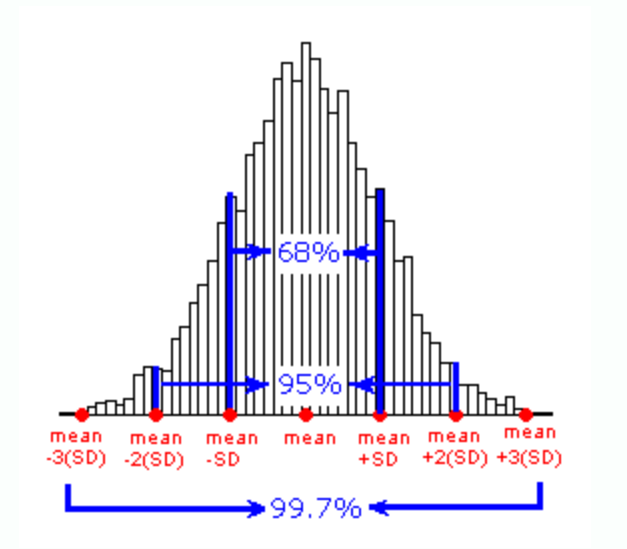
\includegraphics[width=.4\textwidth]{sd.png}
    \caption{An illustration of standard deviation rule.}
\end{figure}
Two variables can be explained as
\begin{itemize}
\item the explanatory variable (also commonly referred to as the independent variable)-—the variable that claims to explain, predict or affect the response; and
\item the response variable (also commonly referred to as the dependent variable)-—the outcome of the study.
\item We should firstly classify the two relevant variables according to their role and type, and only then can we determine what statistical tools should be used to analyze them.
\end{itemize}
C$\rightarrow$C
\begin{itemize}
\item The relationship between two categorical variables is summarized using:
\begin{itemize}
\item Data display: two-way table, supplemented by
\item Numerical summaries: conditional percentages.
\end{itemize}
\item Conditional percentages are calculated for each value of the explanatory variable separately. They can be row percents, if the explanatory variable ``sits'' in the rows, or column percents, if the explanatory variable ``sits'' in the columns.
\item When we try to understand the relationship between two categorical variables, we compare the distributions of the response variable for values of the explanatory variable. In particular, we look at how the pattern of conditional percentages differs between the values of the explanatory variable.
\end{itemize}
$C\rightarrow Q$\\
When exploring the relationship between a categorical explanatory variable and a quantitative response, we essentially compare the distributions of the quantitative response for each category of the explanatory variable using side-by-side boxplots supplemented by descriptive statistics.\\
$Q\rightarrow Q$\\
It is important to mention again that when creating a scatterplot, the explanatory variable should always be plotted on the horizontal X-axis, and the response variable should be plotted on the vertical Y-axis.
Recall that when we described the distribution of a single quantitative variable with a histogram, we described the overall pattern of the distribution (shape, center, spread) and any deviations from that pattern (outliers). We do the same thing with the scatterplot.\\
\begin{figure}
[h!]
\centering
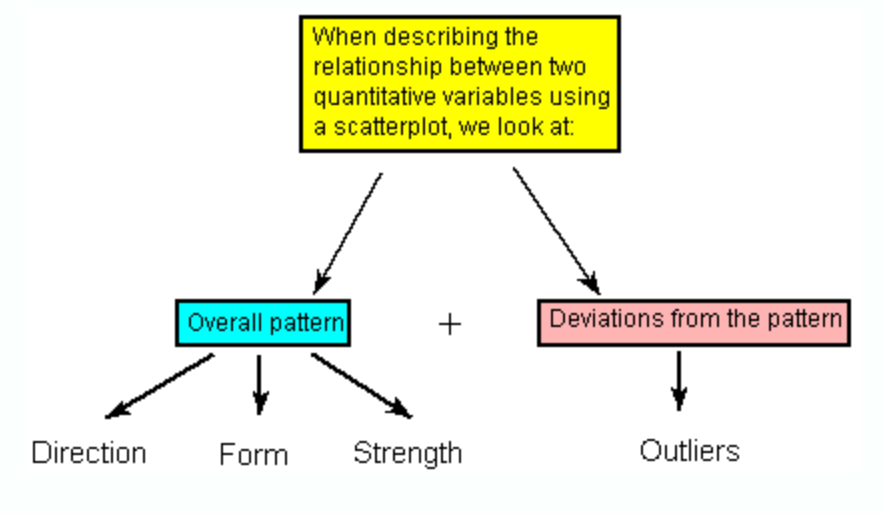
\includegraphics[width=.6\textwidth]{scatter.png}
\caption{An illustration of using scatter plot for explaining distributions.}
\end{figure}
Relationships with a linear form are most simply described as points scattered about a line. 
Relationships with a \textbf{curvilinear} form are most simply described as points dispersed around the same curved line. The \textbf{strength} of the relationship is determined by how closely the data follow the form of the relationship. Data points that deviate from the pattern of the relationship are called \textbf{outliers}.\\
Adding labels to the scatterplot that indicate different groups or categories within the data might help us get more insight about the relationship we are exploring.\\
\subsection{Linear relationships}
The \textbf{correlation coefficient} ($\bm{r}$) is a numerical measure that measures the strength and direction of a linear relationship between two quantitative variables.
\begin{equation}
    \bm{r}={1\over (n-1)}\sum_{i=1}^n 
    \frac{(x_i-\bar{x})(y_i-\bar{y})}
    {\sqrt{\Sigma_{xx}}\sqrt{\Sigma_{yy}}}.
\end{equation}
$\bm{r}\in [-1,1]$. The correlation close to $-1$ indicates a negative relationship between the variables. The correlation close to $+1$ indicates a negative relationship between the variables. The correlation close to $0$ indicates no relationship.\\
Properties:
\begin{enumerate}
\item The correlation does not change when the units of measurement of either one of the variables change. In other words, if we change the units of measurement of the explanatory variable and/or the response variable, the change has no effect on the correlation ($\bm{r}$). In other words, $\bm{r}$ is unitless. 
\item The correlation measures only the strength of a linear relationship between two variables. It \emph{ignores} any other type of relationship, no matter how strong it is. The correlation is useless for assessing the strength of any type of relationship that is not linear.
\item The correlation by itself is not sufficient to determine whether a relationship is linear.
\item The correlation is heavily influenced by outliers.
\end{enumerate}
Least-squares regression
\begin{equation}
Y = a+bX,
\end{equation}
where $\bar{X}$ is the mean of the explantory variable's value, $S_X$ is the standard deviation of the explantory variable value, $\bar{Y}$ is the mean of the response variable's value, $S_Y$ is the standard deviation of the response variable's value and $\bm{r}$ is the correlation coefficient.\\
Then we have 
\begin{align}
  b&=\bm{r}\bigg({S_Y \over S_X}\bigg)\\
  a&=\bar{Y}-b\bar{X}.
\end{align}
The slope of the least squares regression line can be interpreted as the average change in the response variable when the explanatory variable increases by 1 unit.\\
Prediction for ranges of the explanatory variable that are not in the data is called \textbf{extrapolation}. Since there is no way of knowing whether a relationship holds beyond the range of the explanatory variable in the data, extrapolation is not reliable, and should be avoided.\\
\textbf{Principle}: Association \textbf{does not} imply causation!
\subsection{Causality}
\begin{itemize}
\item A \textbf{lurking} variable is a variable that is not among the explanatory or response variables in a study, but could substantially affect your interpretation of the relationship among those variables. \emph{An observed association between two variables is not enough evidence that there is a causal relationship between them.}
\item Whenever including a lurking variable causes us to rethink the direction of an association, this is called Simpson's paradox.
\item A Lurking variable help us to gain a deeper understanding of the relationship between variables, or lead us to rethink the direction of an association.
\item A lurking variable is tied in (or confounded) with the explanatory variable's values, and may itself cause the response to be success or failure. 
\end{itemize}
\section{Producing data}
Exploratory data analysis seeks to illuminate patterns in the data by summarizing the distributions of quantitative or categorical variables, or the relationships between variables. In statistical inference, we will use the summaries about variables or relationships that were obtained in the study to draw conclusions about what is true for the entire population from which the sample was chosen. For this process to ``work'' reliably, it is essential that the sample be truly representative of the larger population.\par
The design for producing data must be considered carefully. Studies should be designed to discover what we want to know about the variables of interest for the individuals in the sample. In particular, if what you want to know about the variables is whether there is a causal relationship between them, special care should be given to the design of the study.\par
A sample that produces data that is not representative because of the systematic under- or over-estimation of the values of the variable of interest is called biased. Bias may result from either a poor sampling plan or from a poor design for evaluating the variable of interest.
Type of samples:
\begin{itemize}
\item Volunteer samples indicate individuals have selected themselves to be included.
\item Convenience sample are individuals happen to be at the right time and place to suit the schedule of the researcher.
\item  The sampling frame of individuals from whom the sample is actually selected should match the population of interest; bias may result if parts of the population are systematically excluded. 
\item Systematic sampling shows that it may not be subject to any clear bias, but it would not be as safe as taking a random sample.
\item A simple random sample (SRS) is if individuals are sampled completely at random, and without replacement, then each group of a given size is just as likely to be selected as all the other groups of that size.
\end{itemize}
Sampling techniques:
\begin{itemize}
\item Simple Random Sampling indicates that each individual as the same chance of being selected.
\item Cluster Sampling --- This sampling technique is used when our population is naturally divided into groups (which we call clusters).
\item Stratified Sampling—Stratified sampling is used when our population is naturally divided into sub-populations, which we call stratum.
\item Difference between Cluster Sampling and Stratified Sampling: In cluster sampling, we take a random sample of whole groups of individuals, while in stratified sampling we take a simple random sample from each group.
\end{itemize}
There is a multi-stage sampling, which perform sampling in steps.\\
Data sampling is the first stage of data production, and now we proceed to the second step of designing studies:
\begin{itemize}
\item Carry out an observational study, in which values of the variable or variables of interest are recorded as they naturally occur. There is no interference by the researchers who conduct the study.
\item Take a sample survey, which is a particular type of observational study in which individuals report variables' values themselves, frequently by giving their opinions.
\item Perform an experiment. Instead of assessing the values of the variables as they naturally occur, the researchers interfere, and they are the ones who assign the values of the explanatory variable to the individuals. The researchers ``take control'' of the values of the explanatory variable because they want to see how changes in the value of the explanatory variable affect the response variable.
\end{itemize}
Here are the types of designing stuides:
\begin{itemize}
    \item a study in which individuals report variable values themselves (frequently their opinions), is a \textbf{survey}.
    \item a \textbf{retrospective observational study} involves recording variables' values that naturally happened in the past.
    \item a \textbf{prospective observational study} records the values of variables as they naturally happen forward in time.
\end{itemize}
\begin{figure}
    [h!]
    \centering
    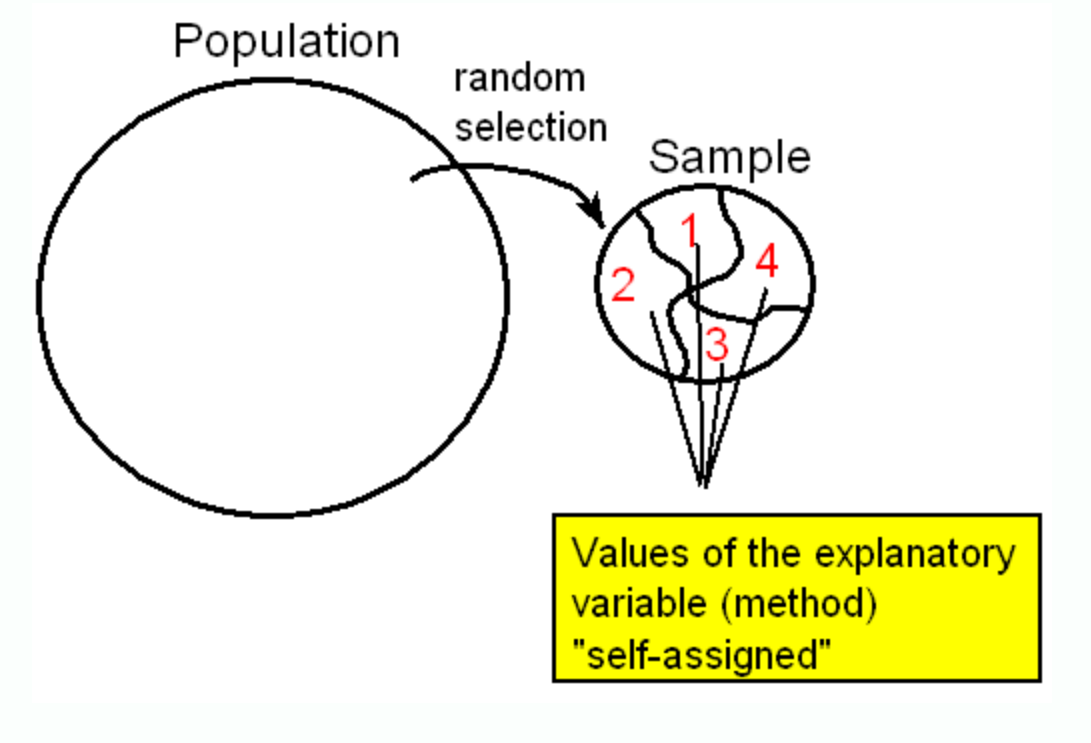
\includegraphics[width=.4\textwidth]{ostudy.png}
    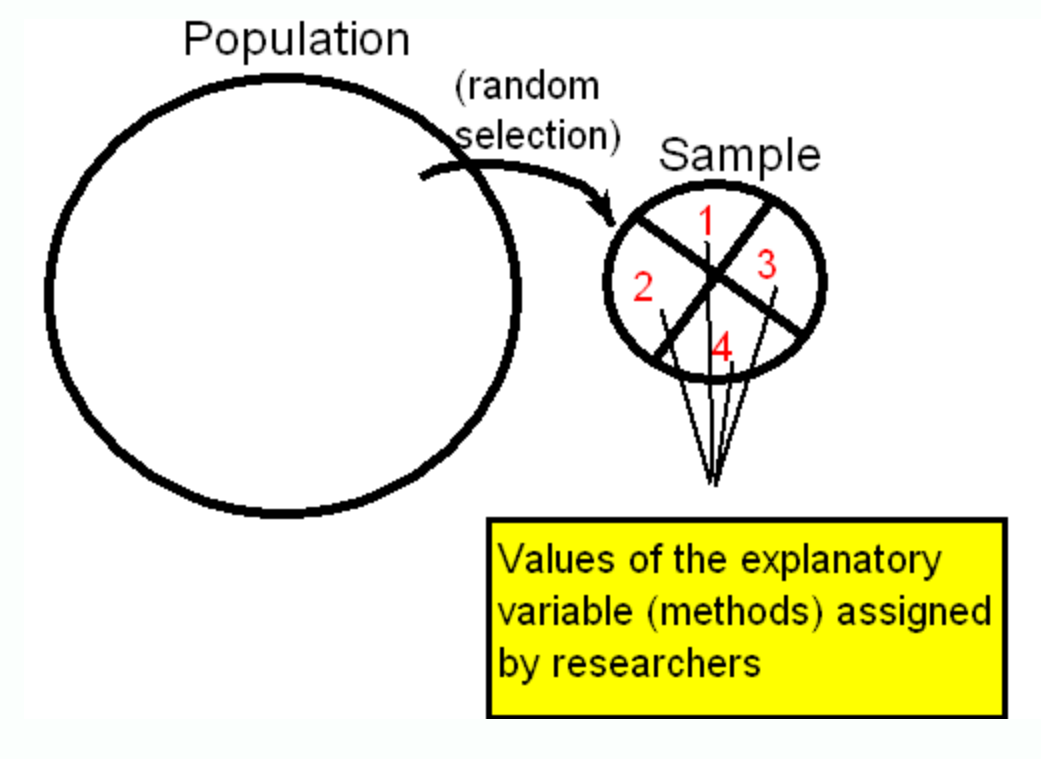
\includegraphics[width=.4\textwidth]{exp.png}
    \caption{A comparison between the observation study and experiment.}
\end{figure}
It is because of the existence of a virtually unlimited number of potential lurking variables that we can never be $100\%$ certain of a claim of causation based on an observational study.\\
Sample surveys include: open vs. closed questions, unbalanced response options, leading questions, planting ideas with questions, complicated questions, sensitive questions.\par
Observational studies:
\begin{itemize}
\item The explanatory variable's values are allowed to occur naturally.
\item Because of the possibility of lurking variables, it is difficult to establish causation.
\item If possible, control for suspected lurking variables by studying groups of similar individuals separately.
\item Some lurking variables are difficult to control for; others may not be identified.
\end{itemize}
Experiments
\begin{itemize}
\item The explanatory variable's values are controlled by researchers (treatment is imposed).
\item Randomized assignment to treatments automatically controls for all lurking variables.
\item Making subjects blind avoids the placebo effect.
\item Making researchers blind avoids conscious or subconscious influences on their subjective assessment of responses.
\item A randomized controlled double-blind experiment is generally optimal for establishing causation.
\item A lack of realism may prevent researchers from generalizing experimental results to real-life situations.
\item Noncompliance may undermine an experiment. A volunteer sample might solve (at least partially) this problem.
\item It is impossible, impractical or unethical to impose some treatments.
\end{itemize}
In order to set up an experiment of more than one explanatory vairables, there has to be one treatment group for every combination of categories of the two explanatory variables.\\
Randomization may be employed at two stages of an experiment: in the selection of subjects, and in the assignment of treatments. The former may be helpful in allowing us to generalize what occurs among our subjects to what would occur in the general population, but the reality of most experimental settings is that a convenience or volunteer sample is used. \\
In some cases, an experiment's design may be enhanced by relaxing the requirement of total randomization and blocking the subjects first, dividing them into groups of individuals who are similar with respect to an outside variable that may be important in the relationship being studied. Blocking in the assignment of subjects is analogous to stratification in sampling.
\begin{figure}
[h!]
\centering
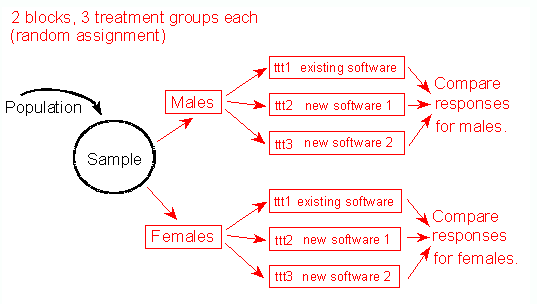
\includegraphics[width=.6\textwidth]{blocking.png}
\caption{An illustration of blocking in Randomization.}
\end{figure}
Such a study design, called matched pairs, may enable us to pinpoint the effects of the explanatory variable by comparing responses for the same individual under two explanatory values, or for two individuals who are as similar as possible except that the first gets one treatment, and the second gets another (or serves as the control). Even though the steps are carried out in this order chronologically, it is generally best for researchers to decide on a study design before they actually obtain the sample. \\ 

\section{Probability}
Probability is the underlying foundation for the methods of statistical inference. We use probability to quantify how much we expect random samples to vary. This gives us a way to draw conclusions about the population in the face of the uncertainty that is generated by the use of a random sample. We can use probability to describe the likelihood that our sample is within a desired level of accuracy. \\
A good example about probabily: Let's Make a Deal. The game is mainly about point out the gift from the box/door, and reveal one from the rest two by the showman. People then should choose the box which is not chosen previously.\\
In general, probability is \emph{not always intuitive}.\\
\emph{Probability} is a mathematical description of randomness and uncertainty. It is a way to measure or quantify uncertainty. Another way to think about probability is that it is the official name for ``chance.'' One way to think of probability is that it is the likelihood that an \emph{event} will occur.
Two fundamental ways to determine probability: theoretical (classical) and empirical (observational). 
\begin{itemize}
\item \emph{Classical} methods are used for games of chance, such as flipping coins, rolling dice, spinning spinners, roulette wheels, or lotteries.
Theoretical methods use the nature of the situation to determine probabilities.
\item Empirical methods use a series of trials that produce outcomes that cannot be predicted in advance (hence the uncertainty).
\end{itemize}
\[
    P(A)=\text{Relative Frequency of Event A} =\frac{\text{numbe of times A occured}}{\text{total number of repetitions}}
\]
Birthday paradox
\[
\displaystyle{p(different) \approx e^{-(n^2 / 2 \cdot T)}}
\]
The above is derived from the Taylor expansion which approximates the non-match between the sequential pairs.
\[
\displaystyle{1 - p(match) \approx e^{-(n^2 / 2 \cdot T)}}
\]
\emph{Law of Large Numbers}: The actual (or true) probability of an event (A) is estimated by the relative frequency with which the event occurs in a long series of trials. The more repetitions that are performed, the closer the relative frequency gets to the true probability of the event.\\
\textbf{Relative Frequency}: 
The probability of an event (A) is the relative frequency with which the event occurs in a long series of trials.
\subsection{Random Variables}
When the outcomes are quantitative, we call the variable a random variable. In statistics, we reserve the term ``random variable'' for quantitative variables. \\
The features of a probability distribution:
\begin{itemize}
\item The outcomes described by the model are random. This means that individual outcomes are uncertain, but there is a regular, predictable distribution of outcomes in a large number of repetitions.
\item The model provides a way of assigning probabilities to all possible outcomes.
\item The probability of each possible outcome can be viewed as the relative frequency of the outcome in a large number of repetitions, so like any other probability, it can be any value between 0 and 1.
\item The sum of the probabilities of all possible outcomes must be 1.
\end{itemize}
Prbability density function \\
Benford's Law states that a set of numbers satisfy that the leading digit $d$ ($d\in \{1,\dots,9\}$) occurs with probability:
\[
  P(d)=log_{10}(d+1)-log_{10}(d)=log_{10}\left(1+{1\over d}\right).
\]
Standardizing Values\\
The first step to assessing a probability associated with a normal value is to determine the relative value with respect to all the other values taken by that normal variable. This is accomplished by determining how many standard deviations below or above the mean that value is. It is described by the z-score mathematically,
\[
    z=\frac{x-\mu}{\sigma}.
\]
The z-scores also allow us to compare values of different normal random variables.\\
A normal table tells the probability of a normal variable taking a value less than any standardized score z.\\
We also get to know that, $Q1=-0.67\sigma$, $\text{med}=0$, $Q3=0.67\sigma$. 
Roughly $25\%$, or one quarter, of a normal variable's values are less than 0.67 standard deviations below the mean. Meanwhile, roughly $75\%$, or three quarters, are less than .67 standard deviations above the mean.
We use the standardized normal variable which is called ``$Z$''.\\
We should know that ``The probability is 0.97 that a worker will spend less than how much money in a week on lunch?'' is equivalent to say that ``What is the 97th percentile for the amount (X) spent by workers in a week for their lunch?''.\\[1mm]
In summary, there are two steps to solving the normal problems:
\begin{enumerate}
\item Given a normal value x, solve for probability:
  \[
    z=\frac{x-\mu}{\sigma}
  \]
\begin{itemize}
\item Standardize: calculate
\item Locate z in the margins of the normal table (ones and tenths for the row, hundredths for the column). Find the corresponding probability (given to four decimal places) of a normal random variable taking a value below z inside the table. (Adjust if the problem involves something other than a "less-than" probability, by invoking either symmetry or the fact that the total area under the normal curve is 1.)
\end{itemize}
\item Given a probability, solve for normal value x:
\begin{itemize}
\item (Adjust if the problem involves something other than a "less-than" probability, by invoking either symmetry or the fact that the total area under the normal curve is 1.) Locate the probability (given to four decimal places) inside the normal table. Find the corresponding z value in the margins (row for ones and tenths, column for hundredths).
\item "Unstandardize": calculate 
  \[
  x=\mu+z\cdot \sigma
  \]
\end{itemize}
\end{enumerate}
\subsection{Sampling distribution}
Sample results change from sample to sample, is called \emph{sampling variability}.\\
A parameter is a number that describes the population; a statistic is a number that is computed from the sample.
\begin{figure}
[h!]
\centering
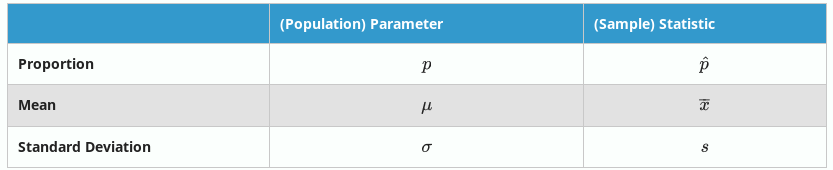
\includegraphics[width=.8\textwidth]{param.png}
\caption{A table summarizes the parameters and statistics.}
\end{figure}
We study the center, spread and shape of the population parameters and statistics, which are also considers as random variables.\\
The sampling distribution for large samples has less variability. $\hat{p}$ has a normal distribution with a mean of $\mu_{\hat{p}}=p$ and the standard deviation $\sigma_{\hat{p}}=\sqrt{\frac{p(1-p)}{n}}$, if $np > 10$ and $n(1-p)>10$.\\
The standard deviation of all sample means ($\bar{x}$) is ${\sigma \over \sqrt{n}}$.\\[1mm]
\textbf{Central Limited Theoreom}: Draw an SRS of size $n$ from any population with mean $m$ and finite standard deviation $s$. When $n$ is large, the sampling distribution of the sample mean $x$ is approximately Normal:
\[
\bar{x}\approx \mathbb{N} \left( \mu, {\sigma \over \sqrt{n}} \right)
\]
Central Limited Theoreom is one of the most important results in introductory statistics. It is stated mathematically as,\\
Suppose $\{X1, X2,\dots\}$ is a sequence of i.i.d. random variables with $E[X_i] = \mu$ and $Var[X_i] = \sigma^2 < \infty$. Then as $n$ approaches infinity, the random variables $\sqrt{n}(S_n − \mu)$ converge in distribution to a normal $N(0, \sigma^2)$:
\begin{equation}
    \sqrt{n} \left( \left( {1 \over n} \sum_{ i = 1}^n X_i \right)-\mu \right) \xrightarrow[]{d} N ( 0 , \sigma^2 ) . 
\end{equation}
Typical problem: We can find the sampling distribution of the sample mean ($\bar{X}$), and use it to learn about the likelihood of getting certain values of $\bar{X}$.\\[1mm]
\subsection{Some summary about probabilty:}
Probability trees are a useful visual tool for displaying and manipulating probabilities of events which naturally happen in sequence (or in stages). It is particularly useful when we are given conditional probability in one direction $P(B | A)$, and need to find the reverse conditional probability $P(A | B)$.\\
\textbf{Random Variables}\\
A random variable is a variable whose values are numerical results of a random experiment.
\begin{itemize}
\item A discrete random variable is summarized by its probability distribution—a list of its possible values and their corresponding probabilities.
  \begin{itemize}
    \item The sum of the probabilities of all possible values must be 1.
    \item The probability distribution can be represented by a table, histogram, or formula.
  \end{itemize}
\item The probability distribution of a random variable can be supplemented with numerical measures of the center and spread of the random variable.
  \begin{itemize}
    \item \textbf{Center}: The center of a random variable is measured by its mean (which is sometimes also referred to as the \textbf{expected value}).
      \begin{enumerate}
      \item The mean of a random variable can be interpreted as its long run average.
      \item The mean is a weighted average of the possible values of the random variable weighted by their corresponding probabilities.
      \item An application of the mean of a random variable is determining premiums for insurance policies.
      \end{enumerate}
    \item \textbf{Spread}: The spread of a random variable is measured by its variance, or more typically by its standard deviation (the square root of the variance).\\
        The standard deviation of a random variable can be interpreted as the typical (or long-run average) distance between the value that the random variable assumes and the mean of X.
\end{itemize}
\item Rules of means and variances give us an easy way to find the mean and standard deviations of the ``new'' random variable $a + bX$ (given the mean and standard deviation of $X$), as well as the mean and standard deviation of the ``new'' random variable $X + Y$ (given the means and standard deviations of $X$ and $Y$, and assuming that $X$ and $Y$ are independent).
\end{itemize}
\textbf{Binomial Random Variables}
\begin{itemize}
\item The binomial random variable is a type of discrete random variable that is quite common.
\item The binomial random variable is defined in a random experiment that consists of n independent trials, each having two possible outcomes (called "success" and "failure"), and each having the same probability of success: p. Such a random experiment is called the binomial random experiment.
\item The binomial random variable represents the number of successes (out of n) in a binomial experiment. It can therefore have values as low as 0 (if none of the n trials was a success) and as high as n (if all n trials were successes).
\item There are "many" binomial random variables, depending on the number of trials (n) and the probability of success (p).
\item The probability distribution of the binomial random variable is given in the form of a formula and can be used to find probabilities. Technology can be used as well.
\item The mean and standard deviation of a binomial random variable can be easily found using short-cut formulas.
\end{itemize}
\textbf{Continuous Random Variables}
The probability distribution of a continuous random variable is represented by a probability density curve. The probability that the random variable takes a value in any interval of interest is the area above this interval and below the density curve.
An important example of a continuous random variable is the normal random variable, whose probability density curve is symmetric (bell-shaped), bulging in the middle and tapering at the ends.
\begin{itemize}
  \item There are "many" normal random variables, each determined by its mean 
(which determines where the density curve is centered) and standard deviation, (which determines how spread out (wide) the normal density curve is).
\item Any normal random variable follows the Standard Deviation Rule, which can help us find probabilities associated with the normal random variable.
\item Another way to find probabilities associated with the normal random variable is using the standard normal table. This process involves finding the z-score of values, which tells us how many standard deviations below or above the mean the value is.
\item An important application of the normal random variable is that it can be used as an approximation of the binomial random variable (under certain conditions). A continuity correction can improve this approximation.
\end{itemize}
\textbf{Sampling Distributions}
A parameter is a number that describes the population, and a statistic is a number that describes the sample.
\begin{itemize}
  \item Parameters are fixed, and in practice, usually unknown.
  \item Statistics change from sample to sample due to sampling variability.
  \item The behavior of the possible values the statistic can take in repeated samples is called the sampling distribution of that statistic.
\end{itemize}
The sampling distribution of the sample proportion, (under certain conditions):
\begin{itemize}
  \item is centered around p, the proportion in the entire population from which the sample is drawn.
  \item has standard deviation of $\sqrt{{p(1-p)\over n}}$.
  \item is approximately normal (under certain conditions).
\end{itemize}
According to the Central Limit Theorem, the sampling distribution of the sample mean, $\bar{X}$:
\begin{itemize}
\item  is centered around $\mu$, the mean in the entire population from which the sample is drawn.
\item has a standard deviation of ${\sigma \over \sqrt{n}}$.
\item is, for a large enough sample size n, approximately normal (regardless of the shape of the population distribution).
\end{itemize}
\section{Statistical inference}
Statistical inference is the process that infers something about the population based on what is measured in the sample.
There are three forms of statistical inference.
\begin{itemize}
  \item In point estimation, we estimate an unknown parameter using a single number that is calculated from the sample data.
  \item In interval estimation, we estimate an unknown parameter using an interval of values that is likely to contain the true value of that parameter (and state how confident we are that this interval indeed captures the true value of the parameter).
  \item In hypothesis testing, we have some claim about the population, and we check whether or not the data obtained from the sample provide evidence against this claim.
  \end{itemize}
  We use statistical inference in two cases:
  \begin{itemize}
    \item When the variable of interest is categorical, the population parameter that we will infer about is the population proportion ($p$) associated with that variable.
    \item When the variable of interest is quantitative, the population parameter that we infer about is the population mean ($\mu$) associated with that variable.  
    \end{itemize}
    $\bar{X}$ is an unbiased estimator of $\mu$, and $\hat{p}$ is an unbiased estimator of $p$. Also note that, point estimates are truly unbiased estimates for the population parameter only if \emph{the sample is random and the study design is not flawed}.\\
    The sampling distribution of the sample mean $\bar{X}$ is, as we mentioned before, centered at the population mean and has a standard deviation of $\frac{\sigma}{\sqrt{n}}$.  This means that values of $\bar{X}$ that are based on a larger sample are more likely to be closer to $\mu$. Similarly, since the sampling distribution of $\hat{p}$ is centered at $p$ and has a standard deviation of $\sqrt{p(1-p)\over n}$, which decreases as the sample size gets larger, values of $\hat{p}$ are more likely to be closer to p when the sample size is larger.\\ 
 The point estimate of the population variance $\sigma^2$ using the sample variance is $s^2=\frac{(x_1-\bar{x})^2+\dots+(x_n-\bar{x})^2}{n-1}$. $s^2$ is an unbiased estimator for $\sigma^2$. Division by $n-1$ accomplishes the goal of making this point estimator unbiased.\\
The idea behind interval estimation is, therefore, to enhance the simple point estimates by supplying information about the size of the error attached.
\subsection{Interval estimation}
Given the fact that we are basing our estimate on one sample that is a small fraction of the population in point estimates, these estimates are in themselves of limited usefulness, unless we can quantify the extent of the estimation error.  Interval estimation addresses this issue. The idea behind \emph{interval estimation} is, to enhance the simple point estimates by supplying information about the size of the error attached.\\
\textbf{Confidence interval}\\
How a $95\%$ confidence interval for the population mean $\mu$ is constructed and interpreted.\\
According to the central limit theorem, the sampling distribution of the sample mean $\bar{X}$ is approximately normal with a mean of $\mu$ and standard deviation of $\sigma \over \sqrt{n}$. We therefore, firstly calculate the sample mean and its std. Then based on the standard deviation rule for the normal distribution, we can obtain the $95\%$ confidence interval ($\bar{x}- 2 \sigma, \; \bar{x}+2 \sigma$) for the mean $\mu$.\\
The interval that we hope that contains the population mean $\mu$ is called an ``interval for the population mean.''  Any normal random variable (in our case $\bar{X}$), has a $95\%$ chance (or probability of .95) of taking a value that is within 2 standard deviations of its mean.\\
\textbf{Connection Between Confidence Intervals and Sampling Distributions}\\
A $99\%$ confidence interval for $\mu$ is $\bar{x} \pm 2.576 \; {\sigma \over \sqrt{n}}$.
A $90\%$ confidence interval for $\mu$ is $\bar{x} \pm 1.645 \; {\sigma \over \sqrt{n}}$.\\
There is a trade-off between the level of confidence and the precision with which the parameter is estimated. When the confidence level increases, the interval becomes wider, i.e. the precision decreaes.\\
\textbf{Understanding the General Structure}\\
We explore the confidence interval for $\mu$ for different levels of confidence and it follows the form:
\begin{equation}
    \bar{x}\pm z^* \cdot {\sigma \over \sqrt{n}},
\end{equation}
where $z^*$ is a general notation for the multiplier thta depend on the level of confidence.
\begin{figure}
    [h!]
    \centering
    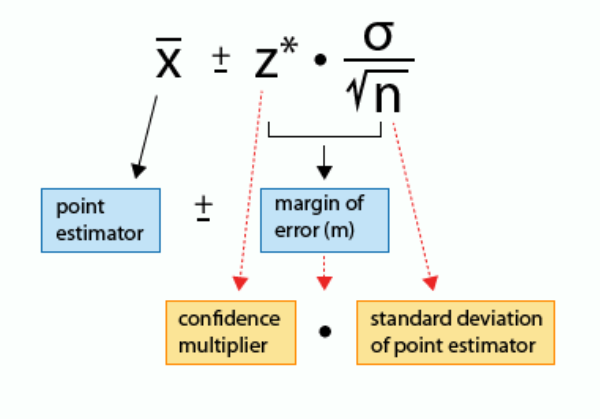
\includegraphics[width=.4\textwidth]{confidence.png}
    \caption{An illustration of the different components of the confidence interval and its structure.}
\end{figure}
The margin of error, $m$, is therefore ``in charge'' of the width (or precision) of the confidence interval, and the estimate is in charge of its location (and has no effect on the width). Also note that $\sigma$ in the margin is a fixed value. 
On an intuitive level, if our estimate $\bar{x}$ is based on a larger sample (i.e., a larger fraction of the population), we have more faith in it, or it is more reliable, and therefore we need to account for less error around it.\\
\textbf{Sample Size calculation}\\
In situations where a researcher has some flexibility as to the sample size, the researcher can calculate in advance what the sample size is that he/she needs in order to be able to report a confidence interval with a certain level of confidence and a certain margin of error.
\begin{equation}
n = \left({z^*\sigma \over m }\right)^2
\end{equation}
From the margin of error, we can determine the number of samples that we need given the margin of error. The sample size should always be an integer. For non-integer results, we should always round up to the next highest integer.\\
If the standard deviation is unknown, we can use the ``range rule of thumb,'' which says that, to a rough approximation, $\sigma$ is no bigger than range/4, where range = max – min. If you have no other estimate for $\sigma$, you can therefore use range/4 as a rough estimate for $\sigma$.\\
One of the most important things to learn with any inference method is the conditions under which it is safe to use it. It is very tempting to apply a certain method, but if the conditions under which this method was developed are not met, then using this method will lead to unreliable results, which can then lead to wrong and/or misleading conclusions. 
First, the sample must be random. Assuming that the sample is random, recall from the Probability unit that the Central Limit Theorem works when the sample size is large (a common rule of thumb for ``large'' is $n > 30$), or, for smaller sample sizes, if it is known that the quantitative variable of interest is distributed normally in the population. The only situation in which we cannot use the confidence interval, then, is when the sample size is small and the variable of interest is not known to have a normal distribution. In that case, other methods, called nonparametric methods.\\
If the population standard deviation $\sigma$ is unknown, we can replace $\sigma$ with the \emph{sample} standard deviation $s$. The bad news is that once $\sigma$ has been replaced by $s$, we \textbf{lose} the Central Limit Theorem, together with the normality of $\bar{X}$, and therefore the confidence multipliers $z^*$ for the different levels of confidence are (generally) not accurate any more. The new multipliers come from a different distribution called the "t distribution" and are therefore denoted by $t^*$ (instead of $z^*$).\\
The confidence interval for the population proportion $p$ is:
\begin{align}
& \hat{p}\pm m \nonumber \\
\Rightarrow \, & \hat{p} \pm z^* \cdot \sqrt{p(1-p)\over n} \nonumber \\
&\text{We replace $p$ with its sample counterpart $\hat{p}$, and work with the standard error of $\hat{p}$, then} \nonumber \\
\Rightarrow \, & \hat{p} \pm z^* \cdot \sqrt{\hat{p}(1-\hat{p})\over n} \nonumber 
\end{align}
\begin{figure}[h!]
\centering
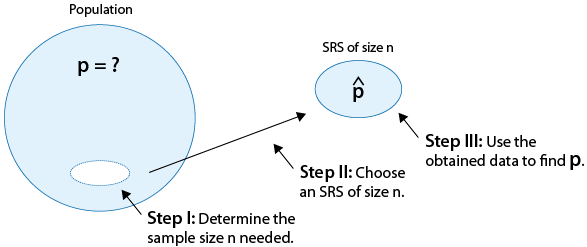
\includegraphics[width=.6\textwidth]{proportion.png}
\caption{Steps to take the point estimation of proportion $p$.}
\end{figure}
From the confidence interval for $p$, we can get that the margin of error is
\begin{equation}
  m=2\sqrt{\hat{p}(1-\hat{p})\over n}\nonumber
\end{equation}
And the the number of samples is
\begin{equation}
  n={4\hat{p}(1-\hat{p})\over m^2}
\end{equation}
But there is a practical problem with this expression that we need to overcome. Practically, you first determine the sample size, then you choose a random sample of that size, and then use the collected data to find $\hat{p}$. So the fact that the expression for determining the sample size depends on $\hat{p}$ is problematic. The way to overcome the problem is to take the conservative approach by setting $\hat{p}={1\over 2}$.\par
It is conservative because the expression that appears in the numerator, is maximized when $\hat{p}={1\over 2}$. That way, the $n$ we get will work in giving us the desired margin of error regardless of what the value of $\hat{p}$ is. This is a ``worst case scenario'' approach. So when we do that we get $n={1\over m^2}$.\par
For media pools, $0.03$ is a very commonly used margin of error. For this reason, most media polls work with a sample of around 1,100 people.\par
Say $m=.01$, the survey has a margin of error of $1\%$. \par
One of the most important things to learn with any inference method is the conditions under which it is safe to use it. It is safe to estimate the sample proportion $\hat{p}$ under the condition that
\begin{equation}
    n\cdot \hat{p}\geq 10; \;\; n \cdot (1-p)\geq 10.\nonumber
\end{equation}
\subsection{Hypothesis testing}
Statistical hypothesis testing is defined as:\\
Assessing evidence provided by the data in favor of or against some claim about the population.\\
There are two types of conclusions:
\begin{itemize}
\item ``The data provide enough evidence to reject claim 1 and accept claim 2''; or
\item ``The data do not provide enough evidence to reject claim 1.''
\end{itemize}
In hypothesis testing, in order to assess the evidence, we need to find how likely is it to get data like those observed assuming that claim 1 is true.\par
\begin{figure}
[h!]
\centering
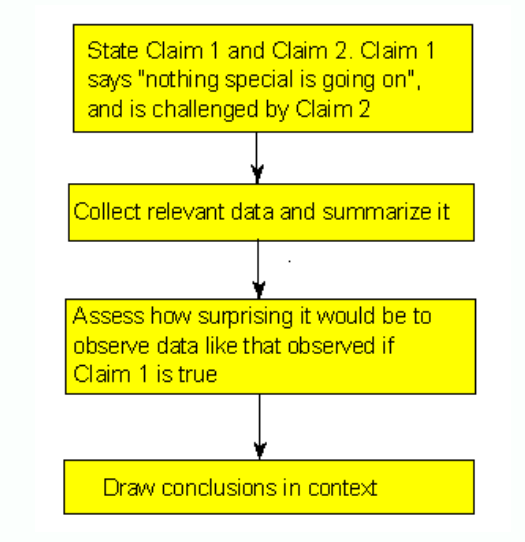
\includegraphics[width=.4\textwidth]{hytest.png}
\caption{An illustration of big picture of statistics.}
\end{figure}
\begin{itemize}
\item Step 1: Stating the claims.\\
In hypothesis testing, Claim 1 is called the null hypothesis (denoted ``$H_0$''), and Claim 2 plays the role of the alternative hypothesis (denoted ``$H_a$''). The null hypothesis suggests nothing special is going on; in other words, there is no change from the status quo, no difference from the traditional state of affairs, no relationship. In contrast, the alternative hypothesis disagrees with this, stating that something is going on, or there is a change from the status quo, or there is a difference from the traditional state of affairs. The alternative hypothesis, $H_a$, usually represents what we want to check or what we suspect is really going on.
\item Step 2: Choosing a sample and collecting data.\\
 You look at sampled data in order to draw conclusions about the entire population. In the case of hypothesis testing, based on the data, you draw conclusions about whether or not there is enough evidence to reject $H_0$.
There is, however, one detail that we would like to add here. In this step we collect data and summarize it. Go back and look at the second step in our three examples. Note that in order to summarize the data we used simple sample statistics such as the sample proportion (
$\hat{p}$), sample mean (
$\bar{x}$) and the sample standard deviation ($s$).
In practice, you go a step further and use these sample statistics to summarize the data with what's called a \emph{test statistic}.
\item Step 3: Assessing the evidence.\\
This is the step where we calculate how likely is it to get data like that observed when $H_0$ true. In a sense, this is the heart of the process, since we draw our conclusions based on this probability. If this probability is very small, then that means that it would be very surprising to get data like that observed if $H_0$ were true. The fact that we did observe such data is therefore evidence against $H_0$, and we should reject it. On the other hand, if this probability is not very small (see example 3) this means that observing data like that observed is not very surprising if $H_0$ were true, so the fact that we observed such data does not provide evidence against $H_0$. This crucial probability, therefore, has a special name. It is called the \textbf{p-value} of the test.\par
The smaller the p-value, the more surprising it is to get data like ours when $H_0$ is true, and therefore, the stronger the evidence the data provide against $H_0$.
\item Step 4: Making conclusions.\\
Since our conclusion is based on how small the p-value is, or in other words, how surprising our data are when Ho is true, it would be nice to have some kind of guideline or cutoff that will help determine how small the p-value must be, or how "rare" (unlikely) our data must be when $H_0$ is true, for us to conclude that we have enough evidence to reject $H_0$.\par
The cutoff is called the significance level of the test and is usually denoted by $\alpha$. The most commonly used significance level is $\alpha$ = 0.05 (or $5\%$). This means that:
\begin{itemize}
\item if the p-value $<\alpha$ (usually 0.05), then the data we got is considered to be "rare (or surprising) enough" when Ho is true, and we say that the data provide significant evidence against Ho, so we reject Ho and accept $H_a$.
\item if the p-value $>\alpha$ (usually 0.05), then our data are not considered to be "surprising enough" when $H_0$ is true, and we say that our data do not provide enough evidence to reject $H_0$ (or, equivalently, that the data do not provide enough evidence to accept $H_a$).
\end{itemize}
\end{itemize}
Terminology:\\
``The results are statistically significant'' - when the p-value  $<\alpha$.\\
``The results are not statistically significant'' - when the p-value  $>\alpha$.\\
\textbf{Note.}\\
\begin{enumerate}
\item The cutoff rate is not the only criterion to decide whether to reject the hypothesis.
\item It is important to draw your conclusions in context. It is never enough to say: ``p-value = \dots, and therefore I have enough evidence to reject Ho at the .05 significance level.''You should always add: ``\dots and conclude that \dots (what it means in the context of the problem)''.
\item There are two types of conclusions:\\
Either I reject $H_0$ and accept $H_a$ (when the p-value is smaller than the significance level) or I cannot reject $H_0$ (when the p-value is larger than the significance level). We never
conclude that we accept the null hypothesis, but just that we cannot
reject it. 
\end{enumerate}
\section{Statistical testing}
Statistical tests is aka significance tests. The first test is about the population proportion ($p$). It is widely known as the \emph{z-test for the population proportion ($p$)}. When we conduct a test about a population proportion, we are working with a categorical variable.\par
\subsection{Stating the hypothesis}
The value that is specified in the null hypothesis is called the \emph{null value}, and is generally denoted by $p_0$. In general, the null hypothesis about the population proportion ($p$) would take the form:
\begin{equation}
    H_0: p = p_0.\nonumber
\end{equation}
$p$ is the unknown population proportion and $p_0$ is the number we think $p$ might be for the given situation.\par
The alternative hypothesis takes one of the following three forms:
\[
    H_a: p < p_0 \text{(one-sided)}
\]
\[
    H_a: p > p_0 \text{(one-sided)}
\]
\[
    H_a: p \neq  p_0 \text{(two-sided)}
\]
The first two possible forms of the alternatives (where the $=$ sign in $H_0$ is challenged by $>$ or $<$) are called \emph{one-sided alternaties}, and the third form of alternative (where the $=$ sign in $H_0$ is challenged by $\neq$) is called a \emph{two-sided alternative}.
\subsection{Collecting and Summarizing the Data (Using a Test Statistic)}
After the hypotheses have been stated, the next step is to obtain a sample (on which the inference will be based), collect relevant data, and summarize them. It is extremely important that our sample is representative of the population about which we want to draw conclusions. This is ensured when the sample is chosen at random.\par
When we summarize the data in hypothesis testing, we go a step beyond calculating the sample statistic and summarize the data with a test statistic. Every test has a test statistic, which to some degree captures the essence of the test. In fact, the p-value is actually determined by (or derived from) the test statistic.\par
The test statistic is a measure of how far the sample proportion $\hat{p}$ is from the null value $p_0$, the value that the null hypothesis claims is the value of $p$. In other words, since $\hat{p}$ is what the data estimates $p$ to be, the test statistic can be viewed as a measure of the ``distance'' between what the data tells us about $p$ and what the null hypothesis claims $p$ to be.\par
We need to standardize the difference $\hat{p}-p_0$ so the comparison between different situations will be possible. The test statistic for this test measures the difference between the sample proportion $\hat{p}$ and the null value $p_0$ by the z-score (standardized score) of the sample proportion $\hat{p}$, assuming that the null hypothesis is true (i.e. assuming that $p=p_0$). Therefore, the test statistic is the z-score of $\hat{p}$ when $p=p_0$, i.e.
\[
    z=\frac{\hat{p}-p_0}{\sqrt{\frac{p_0(1-p_0)}{n}}}.
\]
It represents the difference betweeen the sample proportion ($\hat{p}$) and the null value ($p_0$), measured in standard deviations. It is graphically illustrated in the Figure below.
\begin{figure}
[h!]
    \centering
    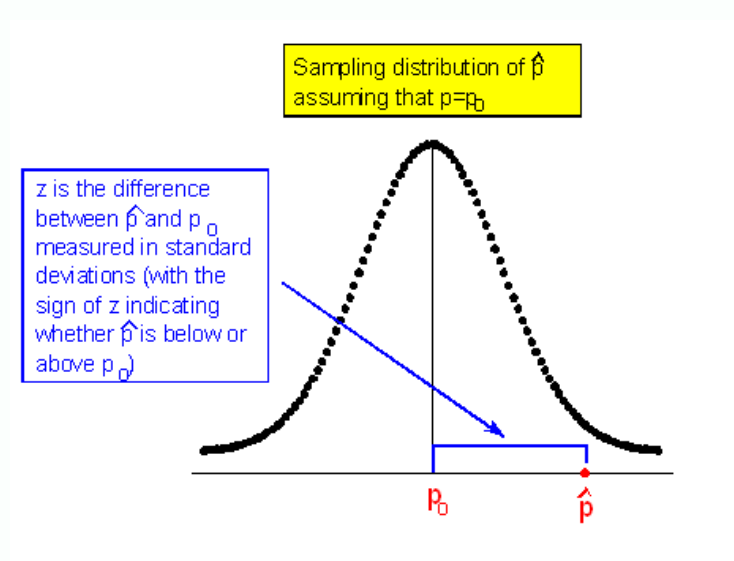
\includegraphics[width=.6\textwidth]{test_stat.png}
    \caption{An illustration of test statistics.}
\end{figure}\\
\textbf{Note.} ``The null distribution of the test statistic is $\mathrm{N}(0,1)$.'' By ``null distribution,'' we mean the distribution under the assumption that $H_0$ is true.\par
Interpretation: Suppose $z=-2$, it means (assuming that $H_0$ is true) the sample proportion is 2 standard deviations below the null value. 
You can also think about this test statistic as a measure of evidence in the data against $H_0$. The larger the test statistic, the ``further the data are from Ho'' and therefore the more evidence the data provide against $H_0$.\par
The results of test statistic hold under two conditions:
\begin{enumerate}
\item The sample has to be random.
\item The conditions under which the sampling distribution of $\hat{p}$ is normal are met. In other words:
\[
n\cdot p_0 \geq 10
\]
\[
n\cdot (1-p_0) \geq 10
\]
\end{enumerate}
We can reiterate the 4 steps of making a hyporthesis test.
\begin{enumerate}
\item State the appropriate null and alternative hypotheses, Ho and Ha.
\item Obtain a random sample, collect relevant data, and check whether the data meet the conditions under which the test can be used. If the conditions are met, summarize the data using a test statistic.
\item Find the p-value of the test.
\item Based on the p-value, decide whether or not the results are significant and draw your conclusions in context.
\end{enumerate}
\subsection{Finding the P-value of the Test}
The \textbf{p-value} is the probability of observing a test statistic as extreme as that observed (or even more extreme) assuming that the null hypothesis is true.
By ``\textbf{extreme}'' we mean extreme in the direction of the alternative hypothesis.\par
When the null hypothesis is true (i.e., when $p=p_0$), the possible values of our test statistic (because it is a z-score) follow a standard normal ($\mathrm{N}(0,1)$, denoted by Z) distribution. Therefore, the p-value calculations (which assume that $H_0$ is true) are simply standard normal distribution calculations for the 3 possible alternative hypotheses.
\begin{enumerate}
\item Less than\\
The probability of observing a test statistic as small as that observed or smaller, assuming that the values of the test statistic follow a standard normal distribution
\[
    H_a: \, p < p_0 \Rightarrow p - \text{value}=P(Z\leq z).
\]
\begin{figure}
    [h!]
    \centering
    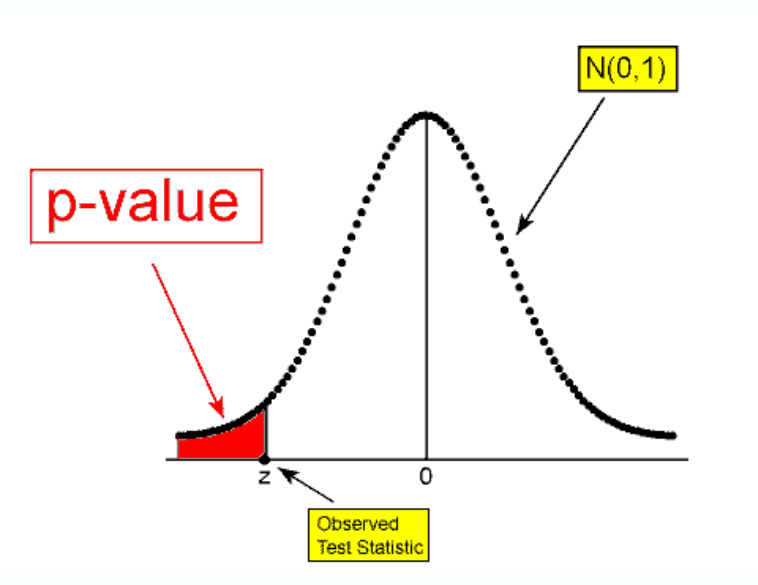
\includegraphics[width=.4\textwidth]{pvalue1.png}
\end{figure}
It is often referred to as a left-tailed test.
\item Greater than\\
The probability of observing a test statistic as large as that observed or larger, assuming that the values of the test statistic follow a standard normal distribution. 
\[
H_a: \, p > p_0 \Rightarrow p - \text{value}=P(Z\geq z).
\]
\begin{figure}
    [h!]
    \centering
    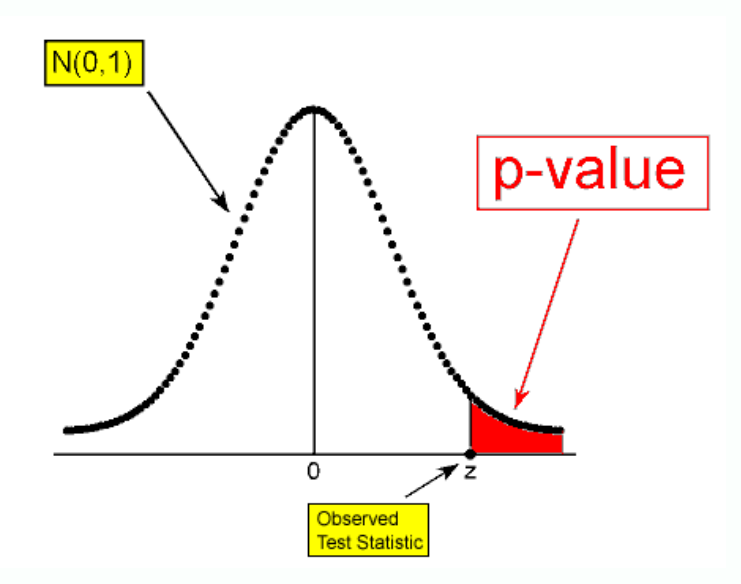
\includegraphics[width=.4\textwidth]{pvalue2.png}
\end{figure}
It is often referred to as a right-tailed test.
\item Not Equal to \\
The probability of observing a test statistic which is as large as in magnitude as that observed or larger, assuming that the values of the test statistic follow a standard normal distribution.
\[
H_a: \, p \neq p_0 \Rightarrow p - \text{value}=P(Z\leq - |z|) + P(Z\geq |z|) = 2\; P(Z \geq |z|).
\]
\begin{figure}
    [h!]
    \centering
    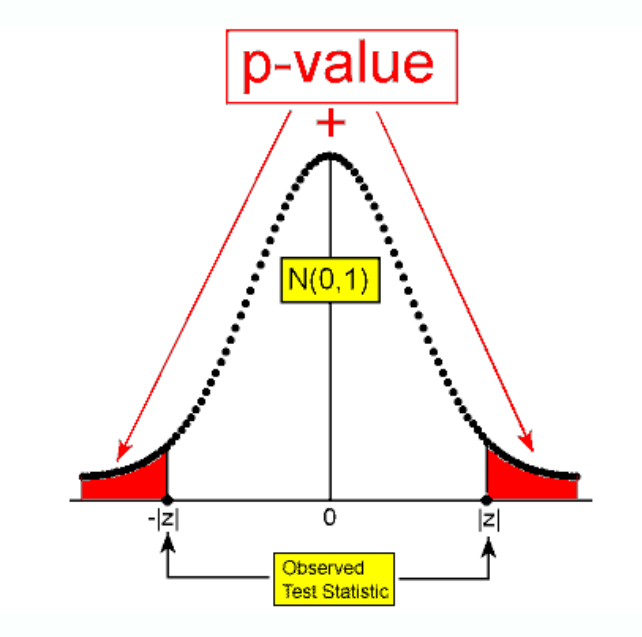
\includegraphics[width=.4\textwidth]{pvalue3.png}
\end{figure}
This is often referred to as a two-tailed test, since we shaded in both directions.\par
Before the widespread use of statistical software, it was common to use 'critical values' instead of p-values to assess the evidence provided by the data. 
\end{enumerate}
\subsection{Concepts of the Critical Value Method}
The critical value is the value, which cuts off an area referred to as the critical region (or area of rejection), as applied to the z test.
\begin{figure}
    [h!]
    \centering
    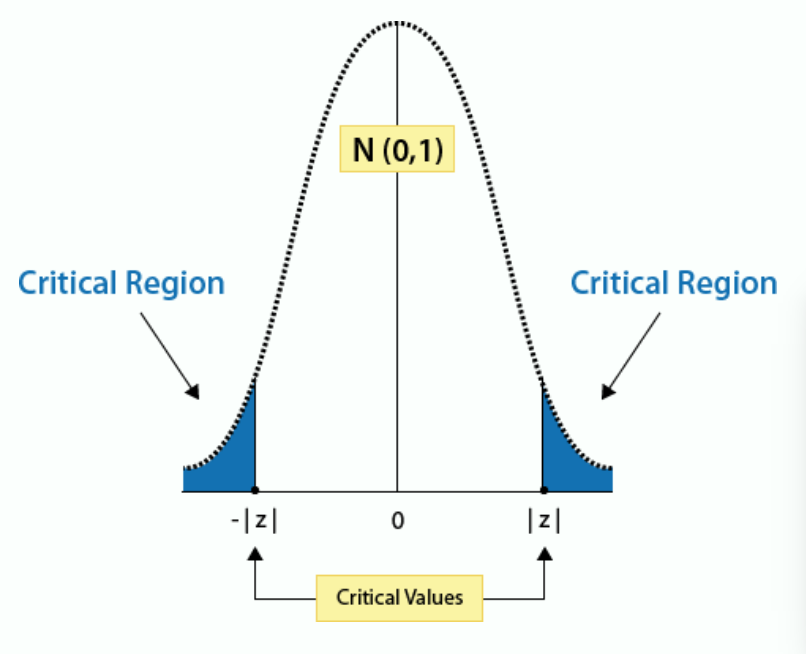
\includegraphics[width=.4\textwidth]{criticalvalue.png}
\end{figure}
When z test statistics fall in the critical region, they are far enough from the mean that they are significantly different from the mean; therefore, in these instances, the null hypothesis would be rejected. The critical region is determined by a critical value that is based on two things: 1) the significance level of the test (either 0.05 or 0.01) AND the direction of the test (ex. left-tailed, right-tailed, or two-tailed).\par
The critical value method uses two concepts: 1) the critical value and 2) the critical region. The critical value is used to determine the critical region and is based on two things: 1) the significance level of the test (either 0.05 or 0.01) AND the direction of the test (ex, left-tailed, right-tailed, or two-tailed).\par
When z-test statistic falls in the critical region, it is far enough from the mean that it is significantly different from the mean. Therefore, in this instance, the null hypothesis would be rejected at the significance level used to determine the critical region (either 0.05 or 0.01). Furthermore, the actual p-value can be determined by using the Normal Table.\par
When the z-test statistic does not fall in the critical region, it indicates that it is not far enough from the mean to be significantly different from the mean. In this instance, the null hypothesis would not be rejected.\par
\textbf{Note.} The critical value method has been traditionally used for hypothesis testing. (There are different critical values and tables for t-tests, ANOVAs, and Chi Square tests). The emphasis now, however, is on the use of exact p-values, which are obtained through the use of statistical software packages.\par
In this case, when $H_0$ is true, the values of the test statistic follow a standard normal distribution (i.e., the sampling distribution of the test statistic when the null hypothesis is true is $\mathrm{N}(0, 1)$). Therefore, p-values correspond to areas (probabilities) under the standard normal curve.
Similarly, in any test, p-values are found using the sampling distribution of the test statistic when the null hypothesis is true (also known as the ``null distribution'' of the test statistic).
\subsection{Drawing Conclusions Based on the P-Value}
\begin{enumerate}
\item Based on the p-value, determine whether or not the results are significant (i.e., the data present enough evidence to reject $H_0$).
\item State your conclusions in the context of the problem.
\end{enumerate}
\subsection{Issues about the Hyporthesis Testing}
\begin{enumerate}
\item The Effect of Sample Size on Hypothesis Testing \\
Larger sample sizes give us more information to pin down the true nature of the population. We can therefore expect the sample mean and sample proportion obtained from a larger sample to be closer to the population mean and proportion, respectively. As a result, for the same level of confidence, we can report a smaller margin of error, and get a narrower confidence interval.
\item Statistical significance vs. practical importance. 
\item One-sided alternative vs. two-sided alternative.\\
We can summarize and say that in general it is harder to reject $H_0$ against a two-sided Ha because the p-value is twice as large. Intuitively, a one-sided alternative gives us a head-start, and on top of that we have the evidence provided by the data. When our alternative is the two-sided test, we get no head-start and all we have are the data, and therefore it is harder to cross the finish line and reject $H_0$.
\item Hypothesis testing and confidence intervals\\ 
Suppose we want to carry out the two-sided test:\\
$H_0:\; p = p_0 $ and $ H_a:\; p \neq p_0$
using a significance level of $0.05$.\\
An alternative way to perform this test is to find a $95\%$ confidence interval for $p$ and check:
\begin{itemize}
\item If falls outside the confidence interval, reject $H_0$.
\item If falls inside the confidence interval, do not reject $H_0$.
\end{itemize}
In other words, if is not one of the plausible values for $p$, we reject $H_0$.\\
If is a plausible value for $p$, we cannot reject $H_0$.\\
If the results are significant, it might be of interest to follow up the tests with a confidence interval in order to get insight into the actual value of the parameter of interest.
\end{enumerate}
\subsection{Hypothesis Testing for the Population Mean}
There are two cases taken into consideration:
\begin{itemize}
\item In the first case ($\sigma$ known), the test is called the z-test for the population mean $\mu$.
\item In the second case ($\sigma$ unknown), the test is called the t-test for the population mean $\mu$.
\end{itemize}
The reason for the different names (z vs. t) is for exactly the same reason that the test for the proportion (p) is called a z-test. In the first case, the test statistic will have a standard normal (z) distribution (when $H_0$ is true), and in the second case, the test statistic will have a t-distribution (when $H_0$ is true).\par
The parameter of interest is the population mean $\mu$ when the variable of interest is quantitative.
\subsection{z-test}
\begin{enumerate}
\item Stating the Hypotheses\\
The null and alternative hypotheses for the z-test for the population mean ($\mu$) have exactly the same structure as the hypotheses for z-test for the population proportion ($p$).
\item Collecting Data and Summarizing Them\\
    The test statistic is the z-score (standardized value) of the sample mean ($\bar{x}$) assuming that $H_0$ is true (in other words, assuming that $\mu = \mu_0$). We refer to results about the sampling distribution of the sample mean ($\bar{X}$), and conclude that sample means behave as follows:
\begin{itemize}
\item Center: The mean of the sample means is µ, the population mean.
\item Spread: The standard deviation of the sample means is ${\sigma \over \sqrt{n}}$.
\item Shape: The sample means are normally distributed if the variable is normally distributed in the population or the sample size is large enough to guarantee approximate normality. Recall that this last statement is the Central Limit Theorem. As a general guideline, we said that if $n > 30$, the Central Limit Theorem applies and we can use a normal curve as a probability model.
\end{itemize}
Based on this description of the sampling distribution of $\bar{X}$, we can define a test statistic that measures the distance between the hypothesized value of $\mu$ (denoted $\mu_0$) and the sample mean (determined by the data) in standard deviation units. It is 
\[
    z = {{\bar{x}-\mu}\over {\sigma \over \sqrt{n}}}.
\]
The Central Limit Theorem gives us criteria for deciding if the z-test for the population mean can be used.\\
\begin{figure}
[h!]
\centering
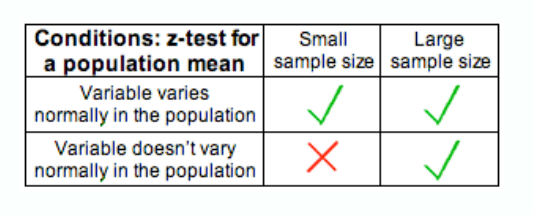
\includegraphics[width=.4\textwidth]{tab_zstat.png}
\end{figure}
When the distribution is extremely skewed to the right, and has one pretty extreme high outlier, we should be cautious to proceed with the statistical testing. It is advisable to take more samples.
\item Finding the p-value of the test\\
The p-value — the probability of getting data (summarized with the test statistic) as extreme as those observed or even more extreme (in the direction of the alternative hypothesis) when $H_0$ is true — for the z-test for the population mean is found exactly like the p-value in the z-test for the population proportion.
\end{enumerate}
\subsection{t-test}
\begin{figure}
[h!]
\centering
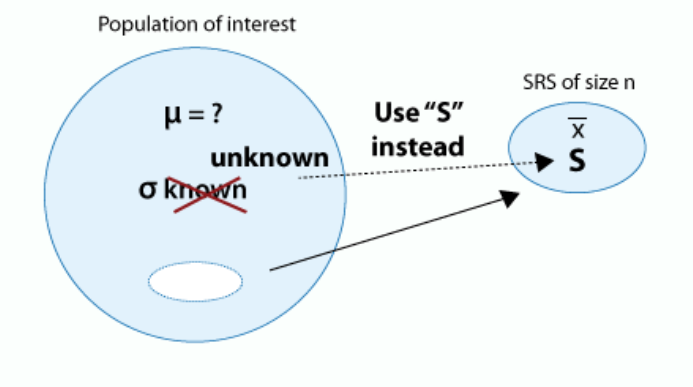
\includegraphics[width=.4\textwidth]{ttest.png}
\end{figure}
As in the z-test, our test statistic will be the standardized score of assuming that ($H_0$ is true). The difference here is that we don't know $\sigma$, so we use $s$ instead. The test statistic for the t-test for the population mean is therefore:
\[
    z = {{\bar{x}-\mu}\over {s \over \sqrt{n}}}.
\]
while in the z-test we divided by the standard deviation of $\bar{X}$, namely $\sigma \over \sqrt{n}$, here we divide by the \textbf{standard error} of $\bar{X}$, namely $s \over \sqrt{n}$.\\
\subsection{The t Distribution}
The t distribution is another bell-shaped (unimodal and symmetric) distribution, like the normal distribution; and the center of the t distribution is standardized at zero, like the center of the normal distribution.\par
The \textbf{spread} in the t distribution is different from the normal distribution.
\begin{figure}
    [h!]
    \centering
    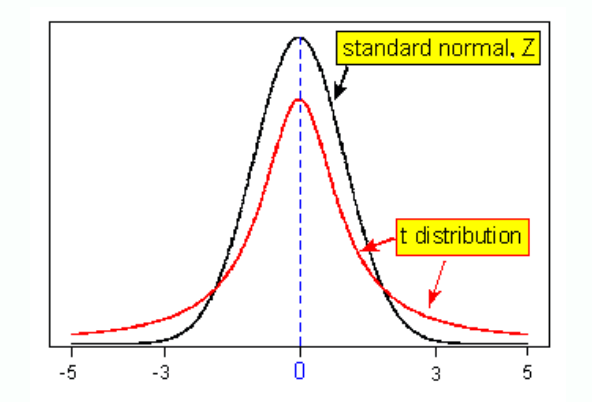
\includegraphics[width=.5\textwidth]{tdistr.png}
\end{figure}
You can see in the picture that the t distribution has slightly less area near the expected central value than the normal distribution does, and you can see that the t distribution has correspondingly more area in the ``tails'' than the normal distribution does. (It is often said that the t distribution has ``fatter tails'' or ``heavier tails'' than the normal distribution.)\par
This reflects the fact that the t distribution has a larger spread than the normal distribution. 
Therefore, the t distribution ends up being the appropriate model in certain cases where there is more variability than would be predicted by the normal distribution. One of these cases is stock values, which have more variability (or ``volatility,'' to use the economic term) than would be predicted by the normal distribution.\par
There's actually an entire family of t distributions.  The t distributions that are closer to normal are said to have higher ``degrees of freedom''.
\begin{figure}
    [h!]
    \centering
    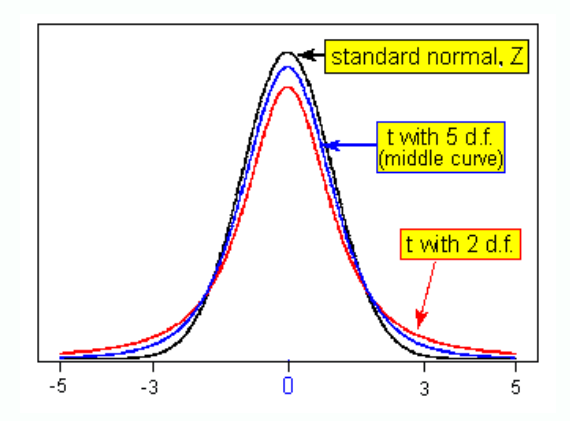
\includegraphics[width=.5\textwidth]{tdistr2.png}
\end{figure}
\subsection{t score}
The test statistic in the test for a mean is 
$t = \frac{\bar{x}- \mu_0}{{s \over \sqrt{n}}}$,
which follows a t distribution.  $s$ (the standard deviation of the sample data) varies from sample to sample, and therefore it is another source of variation. So, using $s$ in place of the standard deviation of the population $\sigma$ causes the sampling distribution to be the t distribution because of that extra source of variation.
\begin{figure}
    [h!]
    \centering
    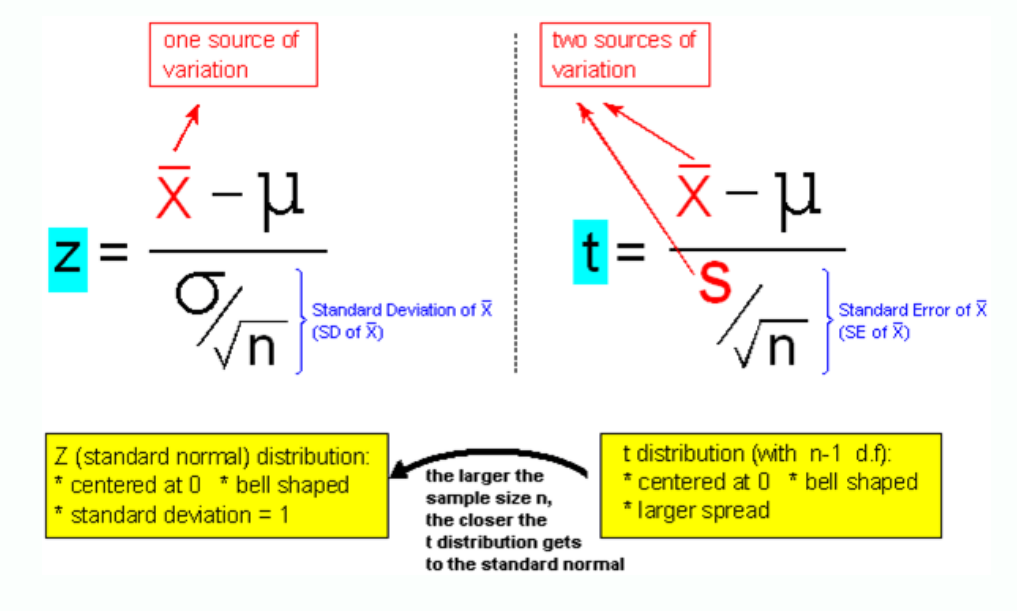
\includegraphics[width=.7\textwidth]{tdistr3.png}
\end{figure}
The t score that arises in the context of a test for a mean is a t score with (n – 1) degrees of freedom. In the context of a test for the mean, the larger the sample size, the higher the degrees of freedom, and the closer the t distribution is to a normal z distribution. The effect of the t distribution is most important for a study with a relatively small sample size.
In summary, we have several conclusions about the t distributon.
\begin{enumerate}
\item  The null distribution of our t-test statistic: 
$t = \frac{\bar{x}- \mu_0}{{s \over \sqrt{n}}}$,
is the t distribution with (n-1) d.f. In other words, when $H_0$ is true (i.e., when
$\mu=\mu_0$), our test statistic has a t distribution with (n-1) d.f., and this is the distribution under which we find p-values.
\item For a large sample size (n), the null distribution of the test statistic is approximately Z, so whether we use t(n - 1) or Z to calculate the p-values should not make a big difference. Here is another practical way to look at this point. If we have a large n, our sample has more information about the population. Therefore, we can expect the sample standard deviation s to be close enough to the population standard deviation, $\sigma$, so that for practical purposes we can use s as the known $\sigma$, and we're back to the z-test.
\end{enumerate}
\textbf{Finding the p-value}\\
The p-value of the t-test is found exactly the same way as it is found for the z-test, except that the t distribution is used instead of the Z distribution.
\begin{figure}
    [h!]
    \centering
    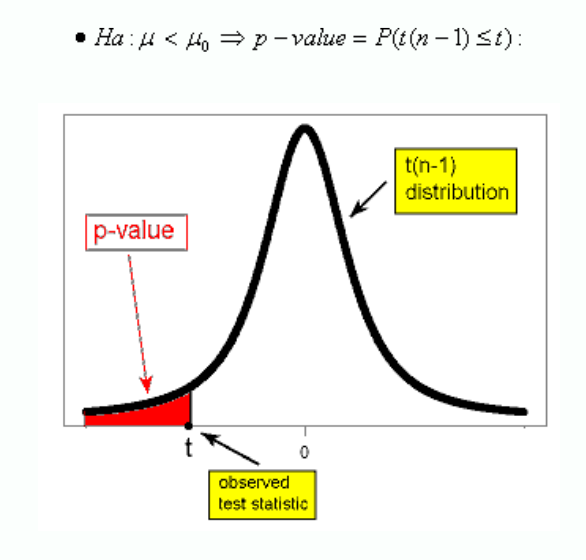
\includegraphics[width=.3\textwidth]{tpvalue1.png}
    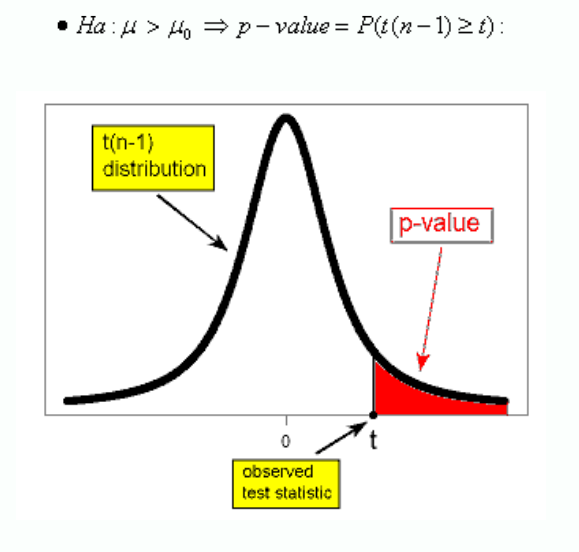
\includegraphics[width=.3\textwidth]{tpvalue2.png}
    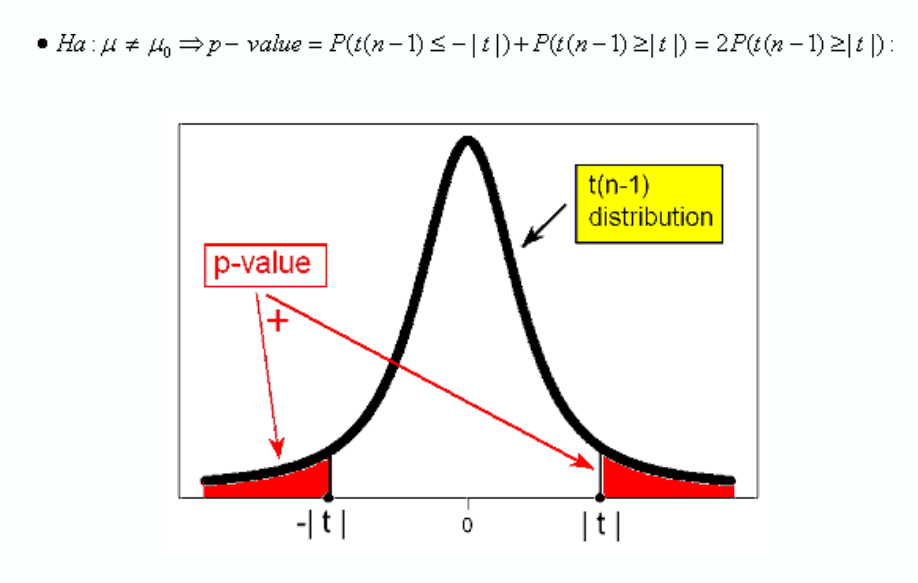
\includegraphics[width=.4\textwidth]{tpvalue3.png}
\end{figure}\\
\textbf{Drawing Conclusions}\\
As usual, based on the p-value (and some significance level of choice) we assess the significance of results, and draw our conclusions in context.\\
To summarize:\\
The main difference between the z-test and the t-test for the population mean is that we use the sample standard deviation s instead of the unknown population standard deviation σ. As a result, the p-values are calculated under the t distribution instead of under the Z distribution.
\subsection{Summary of z-test and t-test}
\begin{enumerate}
\item In hypothesis testing for the population mean ($\mu$), we distinguish between two cases:
\begin{enumerate}
\item The less common case when the population standard deviation (
$\sigma$
 ) is known.
 \item  The more practical case when the population standard deviation is unknown and the sample standard deviation (s) is used instead.
\end{enumerate}
\item In the case when $\sigma$
 is known, the test for is called the z-test, and in case when
 is unknown and s is used instead, the test is called the t-test.
 \item In both cases, the null hypothesis is:
$H_0: \; \mu_0=\mu$
 and the alternative, depending on the context, is one of the following:
 $H_a\;:\; \mu < \mu_0 $, or  $H_a\;:\; \mu > \mu_0 $, or $H_a\;:\; \mu \neq \mu_0 $
 \item  Both tests can be safely used as long as the following two conditions are met:
\item  The sample is random (or can at least be considered random in context).
\item  Either the sample size is large ($n > 30$) or, if not, the variable of interest can be assumed to vary normally in the population.
\end{enumerate}
\begin{enumerate}
\item 
 In the z-test, the test statistic is:
 $z=\frac{\bar{X}-\mu_0}{{\sigma \over \sqrt{n}}}$.
 whose null distribution is the standard normal distribution (under which the p-values are calculated).
\item In the t-test, the test statistic is:
    $t=\frac{\bar{X}-\mu_0}{{s \over \sqrt{n}}}$.
whose null distribution is $t(n - 1)$ (under which the p-values are calculated).
\item  For large sample sizes, the z-test is a good approximation for the t-test.
\item Confidence intervals can be used to carry out the two-sided test
\[
    H_0: \mu = \mu_0 \, \text{vs.} \, H_0: \mu \neq \mu_0 
\]
and in cases where $H_0$ is rejected, the confidence interval can give insight into the value of the population mean ($\mu$.)
\item Here is a summary of which test to use under which conditions:
\begin{figure}
    [h!]
    \centering
    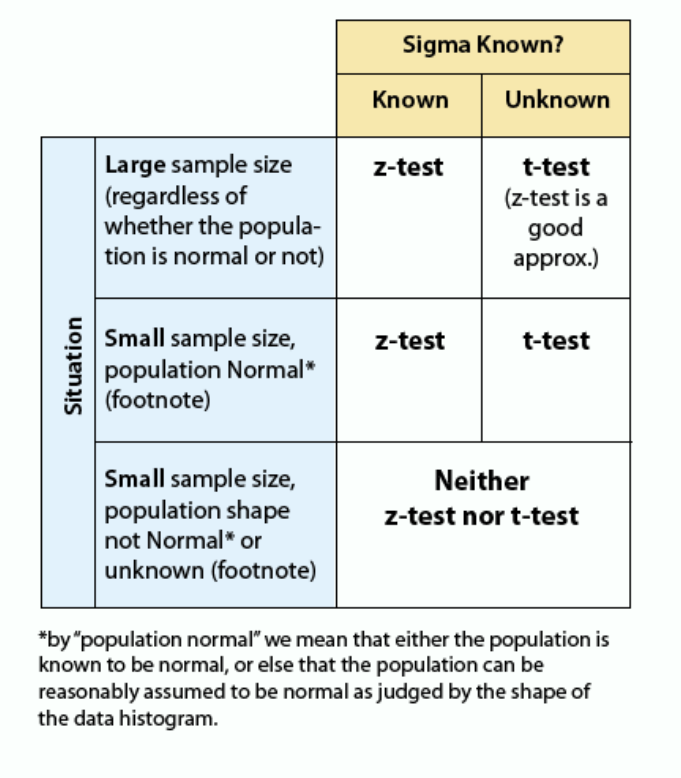
\includegraphics[width=.4\textwidth]{zttest.png}
\end{figure}
\end{enumerate}
In hypothesis testing, the following decisions can occur:
\begin{itemize}
\item If the null hypothesis is true and we do not reject it, it is a correct decision.
\item If the null hypothesis is false and we reject it, it is a correct decision.
\item If the null hypothesis is true, but we reject it. This is a type I error.
\item If the null hypothesis is false, but we fail to reject it. This is a type II error.
\end{itemize}
Type I and type II errors are not caused by mistakes. They are the result of random chance. The data provide evidence for a conclusion that is false.\par
The smaller significance level $\alpha$ is, the smaller the probability of a type I error there will be. 
It is more complicated to calculate the probability of a type II error. The best way to reduce the probability of a type II error is to increase the sample size. But once the sample size is set, larger values of α will decrease the probability of a type II error while increasing the probability of a type I error.\\
\textbf{General guidelines for choosing a level of significance:}
\begin{itemize}
\item If the consequences of a type I error are more serious, choose a small level of significance ($\alpha$).
\item If the consequences of a type II error are more serious, choose a larger level of significance ($\alpha$). But remember that the level of significance is the probability of committing a type I error.
\item In general, we choose the largest level of significance that we can tolerate as the chance of making a type I error.
\end{itemize}
Note: It is not always the case that one type of error is worse than the other.
\section{Inference for relationships}
There are three major forms of inference:
\begin{itemize}
\item Point estimation---estimating an unknown parameter with a single value that is computed from the sample.
\item Interval estimation---estimating an unknown parameter by an interval of plausible values. To each such interval we attach a level of confidence that indeed the interval captures the value of the unknown parameter and hence the name confidence intervals.
\item Hypothesis testing---a four-step process in which we are assessing evidence provided by the data in favor or against some claim about the population parameter.
\end{itemize}
Our goal is to perform inference about relationships between two variables in a population, based on an observed relationship between variables in a sample. 
\begin{figure}
[h!]
\centering
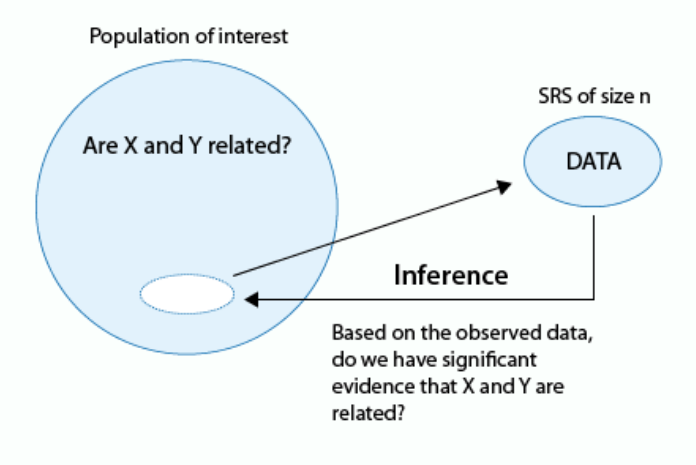
\includegraphics[width=.4\textwidth]{infer1.png}
\end{figure}
The primary method of investigation is hypothesis testing. We will test the form of:
\begin{itemize}
\item $H_0:$ There is no relationship between $X$ and $Y$.
\item $H_a:$ There is a siginificant relationship between $X$ and $Y$.
\end{itemize}
\subsection{Case C $\rightarrow$ Q}
Within the sub-case of comparing two means (i.e., examining the relationship between X and Y, when X has only two categories) we will distinguish between two (sub-sub) cases. The distinction is what study design will be implemented.  \\
\textbf{Two independent samples}\\
In some cases, one group (sub-population 1) has one categorical value, and another independent group (sub-population 2) has the other value. Independent samples are then taken from each group for comparison.\par
Our goal is to test whether the means $\mu_1$ and $\mu_2$ (which are the means of the variable of interest in the two sub-populations) are equal or not, and in order to do that we have two samples, one from each sub-population, which were chosen independently of each other. \\
\begin{figure}
[h!]
\centering
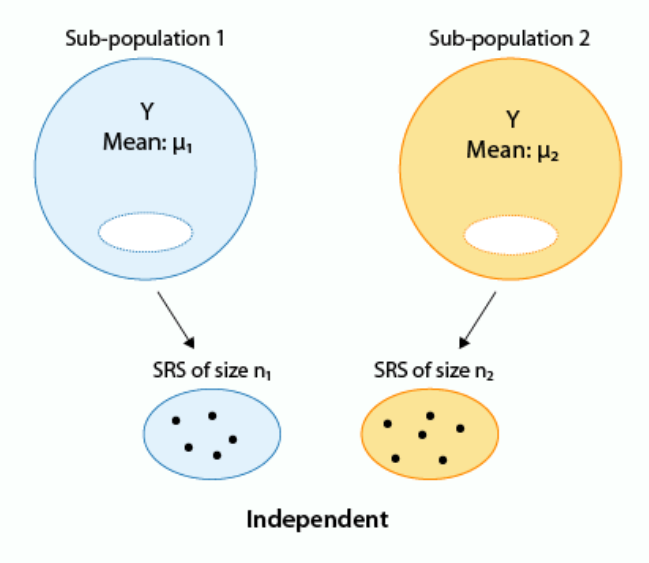
\includegraphics[width=.4\textwidth]{infer2.png}
\end{figure}\\
We will perform the \textbf{two-sample t-test}.
\begin{enumerate}
\item The hypotheses represent our goal, comparing the means: $\mu_1$ and $\mu_2$. \\
Null hypothesis: $H_0: \, \mu_1 - \mu_2 = 0 $\\
Alternative hypothesis: \\
$H_a: \, \mu_1 - \mu_2 > 0 $\\
$H_a: \, \mu_1 - \mu_2 < 0 $\\
$H_a: \, \mu_1 - \mu_2 \neq 0 $\\
\item Check Conditions, and Summarize the Data Using a Test Statistic\\
The two-sample t-test can be safely used as long as the following conditions are met:
\begin{itemize}
\item  The two-sample t-test can be safely used as long as the following conditions are met:
\item The two-sample t-test can be safely used when the samples are independent and at least one of the following two conditions hold:  
\begin{itemize}
\item Both populations are normal, or more specifically, the distribution of the response Y in both populations is normal, and both samples are random (or at least can be considered as such).  
\item The populations are known or discovered not to be normal, but the sample size of each of the random samples is large enough (we can use the rule of thumb that $> 30$ is considered large enough).
\end{itemize}
\item Finding the p-value
\item Conclusion in context\\
P-values are obtained from the output, and conclusions are drawn as usual, comparing the p-value to the significance level alpha.
\item Two-Sample t Confidence Interval\\
A $95\%$ confidence interval which will provide us with a set of plausible values for the difference between the population means $\mu_1-\mu_2$. In particular, if the test has rejected $H_0: \, \mu_1 - \mu_2 = 0$, a confidence interval for $\mu_1-\mu_2$ can be insightful since it quantifies the effect that the categorical explanatory variable has on the response. The $95\%$ confidence interval for $\mu_1-\mu_2$ is 
\[
    (\bar{Y}_1 - \bar{Y}_2) \pm t^* \sqrt{\frac{s_1^2}{n_1} + \frac{s^2_2}{n_2}}.
\]
\end{itemize}
The two-sample t-test statistic is:
\[
    t = \frac{\bar{Y}_1 - \bar{Y}_2}{{s_1^2 \over n_1} + {s_2^2 \over n_2}}.
\]
Where
$\bar{Y}_1$, $\bar{Y}_2$ are the sample means of the samples from population 1 and population 2, respectively.\\
$s_1$, $s_2$ are the sample standard deviation of the samples from population 1 and population 2, respectively.\\
$n_1$, $n_2$ are the sample sizes. \\
\textbf{Interpretation of the inference $\mu_1-\mu_2$.}
\begin{itemize}
\item $\bar{y}_1$ estimates $\mu_1$, $\bar{y}_2$ estimates $\mu_2$, and therefore $\bar{y}_1 - \bar{y}_2$ is what the data tells us about $\mu_1-\mu_2$.
\item 0 is the ``null value'' --- what the null hypothesis, $H_0$ claims that $\mu_1-\mu_2$ is.
\item The denominator ${{s_1^2 \over n_1} + {s_2^2 \over n_2}}$ is the standard error of $\bar{y}_1 - \bar{y}_2$ .\\
Therefore, we can see that our test statistic has the structure.
\[
\frac{\text{sample estimate - null value}}{\text{standard error}}.
\]
It measures (in standard errors) the difference between what the data tell us about the parameter of interest (sample estimate) and what the null hypothesis claims the value of the parameter is (null value).
\end{itemize}
\end{enumerate}
\textbf{Matched pairs}\\
In other cases, a matched pair sample design may be used, where each observation in one sample is matched/paired/linked with an observation in the other sample. These are sometimes called ``dependent samples.'' Matching could be by person (if the same person is measured twice), or could actually be a pair of individuals who belong together in a relevant way (husband and wife, siblings). In this design, then, the same individual or a matched pair of individuals is used to make two measurements of the response---one for each of the two categorical values. One common case is paired by subject.\par
Note that in the first figure, where the samples are independent, the sample sizes of the two independent samples need not be the same (and thus we used $n_1$ and $n_2$ to indicate the two sample sizes). On the other hand, it is obvious from the design that in the matched pairs the sample sizes of the two samples must be the same (and thus we used $n$ for both).  The samples are \textbf{dependent}.
\begin{figure}
[h!]
\centering
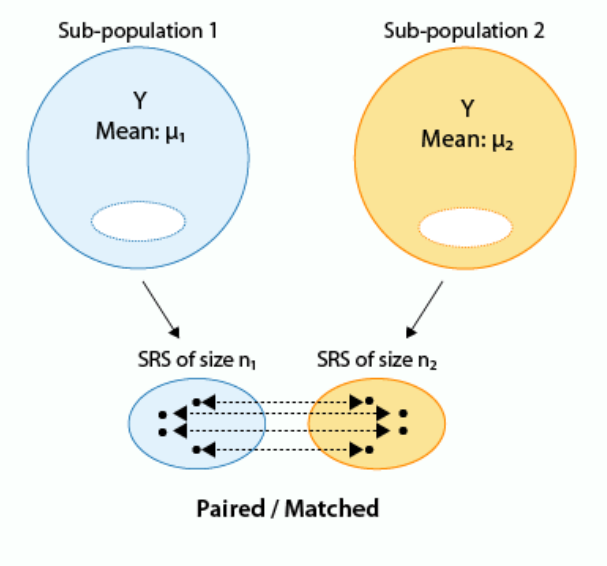
\includegraphics[width=.4\textwidth]{infer3.png}
\end{figure}\\
\begin{enumerate}
\item Stating the hypotheses. \\
The nul hypothesis is always
\[
H_0:\, \mu_d = 0.
\]
And the alternative is one of:
\[
    H_a: \, \mu_d < 0. \text{(One-sided)}
\]
\[
    H_a: \, \mu_d > 0. \text{(One-sided)}
\]
\[
    H_a: \, \mu_d \neq 0. \text{(Two-sided)}
\]
depending on the context.
\item Checking Conditions and Calculating the Test Statistic\\
The paired t-test, as a special case of a one-sample t-test, can be safely used as long as:
\begin{itemize}
\item  The sample of differences is random (or at least can be considered so in context).
\item We are in one of the three situations marked with a green check mark in the following table. The data should not display any departure from the normality assumption in the form of extreme skewness and/or outliers.
\end{itemize}
Assuming that the we can safely use the paired t-test, the data are summarized by a test statistic:
\[
t = \frac{\bar{x}_d - 0}{{s_d \over \sqrt{n}}},
\]
where $\bar{x}_d$ is the sample mean of the differences, and $s_d$is the sample standard deviation of the differences. It measures (in standard errors) how far our data are (represented by the average of the differences) from the null hypothesis (represented by the null value, 0).
\item Finding the p-value\\
As a special case of the one-sample t-test, the null distribution of the paired t-test statistic is a t distribution (with n - 1 degrees of freedom), which is the distribution under which the p-values are calculated. 
\item Conclusion in Context \\
We draw our conclusion based on the p-value. If the p-value is small, there is a significant difference between what was observed in the sample and what was claimed in $H_0$, so we reject $H_0$ and conclude that the categorical explanatory variable does affect the quantitative response variable as specified in $H_a$. If the p-value is not small, we do not have enough statistical evidence to reject $H_0$. In particular, if a cutoff probability, $\alpha$ (significance level), is specified, we reject $H_0$ if the p-value is less than $\alpha$. Otherwise, we do not reject $H_0$.
\item Paired t Confidence Interval\\
If $H_0$ is rejected, a $95\%$ confidence interval for μd can be very insightful and can also be used for the two-sided test.
\end{enumerate}
\textbf{Comparing More Than Two Means---ANOVA}\\
We make inferences about the relationship between the explanatory (X) and the response (Y) variables amounts to comparing the means of the response variable in the populations defined by the values of the explanatory variable, where the number of means we are comparing depends on the number of values of X. Unlike the two-valued case, where we looked at two sub-cases (1) when the samples are independent (two samples design) and (2) when the samples are dependent (matched pairs design, here, we are just going to discuss the case where the samples are independent.\par 
The inferential method for comparing more than two means from independent samples is called Analysis Of Variance (abbreviated as ANOVA), and the test associated with this method is called the ANOVA F-test.
The extension of the matched pairs design to more than two dependent samples is called ``Repeated Measures''\par
\begin{figure}
[h!]
\centering
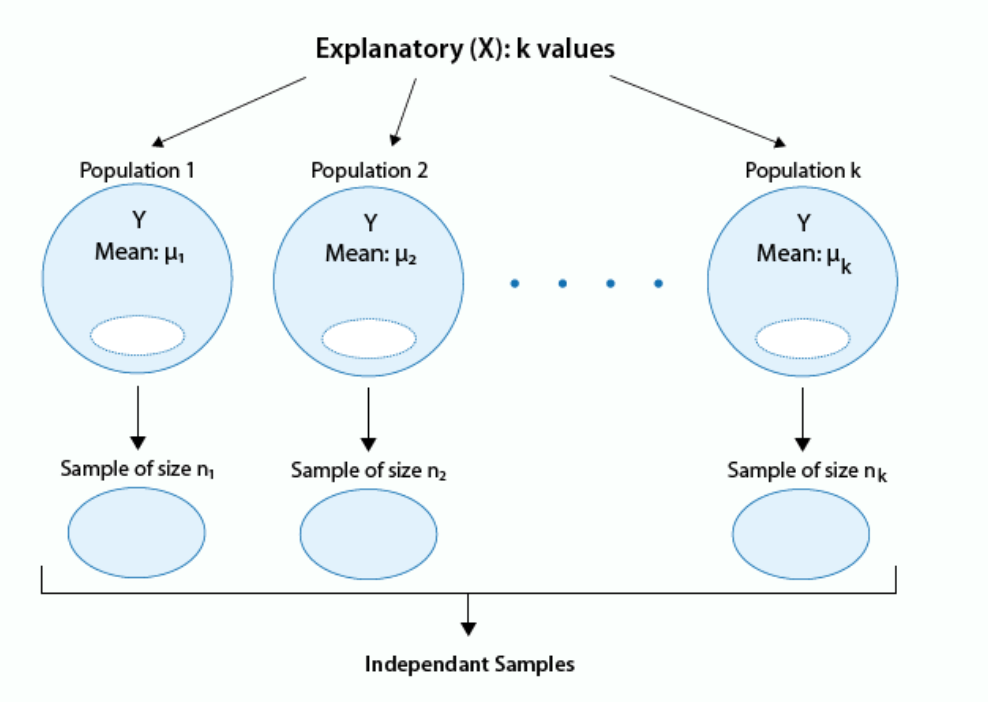
\includegraphics[width=.7\textwidth]{infermulti1.png}
\end{figure}
\begin{enumerate}
\item Stating the Hypotheses\\ 
We discuss about ANOVA in the following:\\
The null hypothesis claims that there is no relationship between X and Y. The null hypothesis of the F-test is:\\ 
\[H_0:\, \mu_1=\mu_2=\dots=\mu_k.\]
Alternative hypothesis claims that there is a relationship between X and Y. In terms of the means , it simply says the opposite of the alternative, that not all the means are equal, and we simply write:
\[
    H_a: \, \text{not all the }\mu\text{'s are equal}.
\]
\textbf{The idea behind the ANOVA F-Test}\\
The question we want to ask from the F-Test is: Are the differences among the sample means ($\bar{Y}$'s) due to true differences among the $\mu$'s (alternative hypothesis), or merely due to sampling variability (null hypothesis)?\par 
We check the quantity:
\[
    \frac{\text{Variation among sample means}}{\text{Variation within groups}}
\]
\item Checking Conditions and Finding the Test Statistic\\
The sample is chosen at random, so the samples are independent. If the sample sizes are quite low, then we need to check whether the boxplots display any extreme violation of the normality assumption in the form of extreme skewness or outliers.
We can assume that the equal population standard deviation condition is met, since the rule of thumb is satisfied (max std / min std is less than 2).\par
The ``F-test'' part comes from the fact that the null distribution of the test statistic, under which the p-values are calculated, is called an F-distribution.\par
It is fairly straightforward to decide if a z-statistic is large. Even without tables, we should realize by now that a z-statistic of 0.8 is not especially large, whereas a z-statistic of 2.5 is large. In the case of the t-statistic, it is less straightforward, because there is a different t-distribution for every sample size n (and degrees of freedom n - 1). However, the fact that a t-distribution with a large number of degrees of freedom is very close to the Z (standard normal) distribution can help to assess the magnitude of the t-test statistic.\par
When the size of the F-statistic must be assessed, the task is even more complicated, because there is a different F-distribution for every combination of the number of groups we are comparing and the total sample size. We will nevertheless say that for most situations, an F-statistic greater than 4 would be considered rather large, but tables or software are needed to get a truly accurate assessment.
\item Finding the p-value\\
The p-value of the ANOVA F-test is the probability of getting an F statistic as large as we got (or even larger), had $H_0: \, \mu_1=\mu_2=\dots=\mu_k$
been true. In other words, it tells us how surprising it is to find data like those observed, assuming that there is no difference among the population means $\mu_1, \mu_2, \dots, \mu_k$.
\item Making Conclusions in Context
\item 
If the ANOVA F-test has rejected the null hypothesis we can look at the confidence intervals for the population means that are in the output to get a visual insight into why $H_0$ was rejected (i.e., which of the means differ).
\end{enumerate}
\subsection{Case $ C\rightarrow C$ }
We aim to assess whether the relationship between X and Y that we observed in the data is due to a real relationship between X and Y in the population or if it is something that could have happened just by chance due to sampling variability.\par
The statistical test is called the $\chi^2$ test for independence.
\begin{enumerate}
\item Stating the hypotheses\\
$H_0$: There is no relationship between the two categorical variables. (They are independent.)\\
$H_a$: There is a relationship between the two categorical variables. (They are not independent.)\\
The idea behind the $\chi^2$ test is to measure how far the data are from what is claimed in the null hypothesis.\\
We will have two sets of counts:
\begin{itemize}
\item the observed counts (the data)
\item the expected counts (if Ho were true)
\end{itemize}
We will measure how far the observed counts are from the expected ones. In other words, we will base our decision on the size of the discrepancy between what we observed and what we would expect to observe if $H_0$ were true. Based on the rule that,  if events $A$ and $B$ are independent, then $P(A, B) = P(A) \cdot P(B)$.\\
The expected count from the table is:
\[
    \text{Expect Count} = \frac{\text{Column Total} \cdot \text{Row Total}}
    {\text{Table Total}}
\]
\item Checking the Conditions and Calculating the Test Statistic \\
The single number that summarizes the overall difference between observed and expected counts is the chi-square statistic $\chi^2$, which tells us in a standardized way how far what we observed (data) is from what would be expected if $H_0$ were true.
\[
    \chi^2 = \sum_{\text{all cells}}\frac{(\text{Observed Count} - \text{Expected Count})^2}
    {\text{Expected Count}}
\]
The reason we divide each square difference by the expected counts is so that the null distribution of $\chi^2$ will have a known null distribution (under which p-values can be easily calculated).
\item Conditions under Which the Chi-Square Test Can Safely Be Used
\begin{itemize}
    \item The sample should be random.
    \item In general, the larger the sample, the more accurate and reliable the test results are. There are different versions of what the conditions are that will ensure reliable use of the test, all of which involve the expected counts. One version of the conditions says that all expected counts need to be greater than 1, and at least $80\%$ of expected counts need to be greater than 5. A more conservative version requires that all expected counts are larger than 5.
\begin{figure}
[h!]
\centering
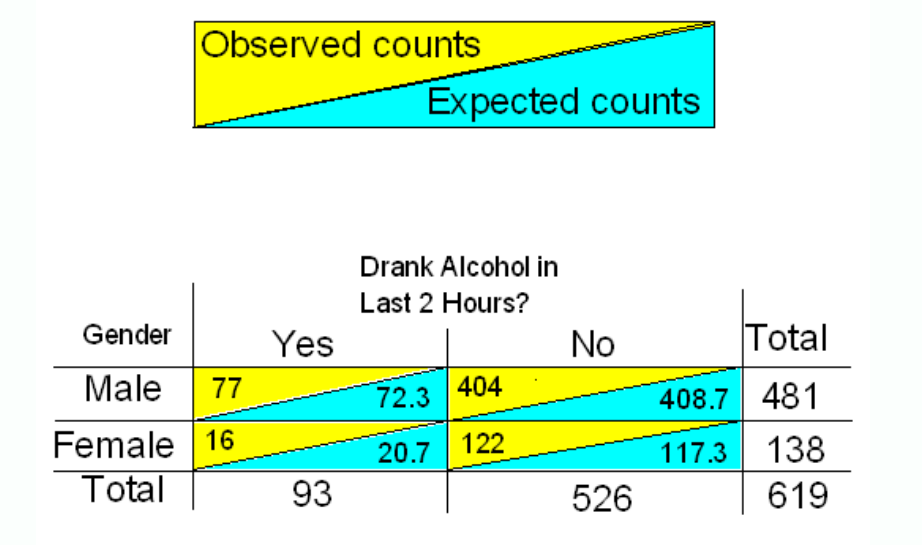
\includegraphics[width=.5\textwidth]{infercc1.png}
\end{figure}
\item Finding the p-value\\
The p-value for the chi-square test for independence is the probability of getting counts. Technically, the p-value is the probability of observing at least as large as the one observed.
\item  Stating the conclusion in context\\
If a significance level of 0.05 is used, we will reject Ho if the p-value is less than 0.05.
\end{itemize}
\end{enumerate}
\subsection{Case $ Q\rightarrow Q$}
\begin{figure}
[h!]
\centering
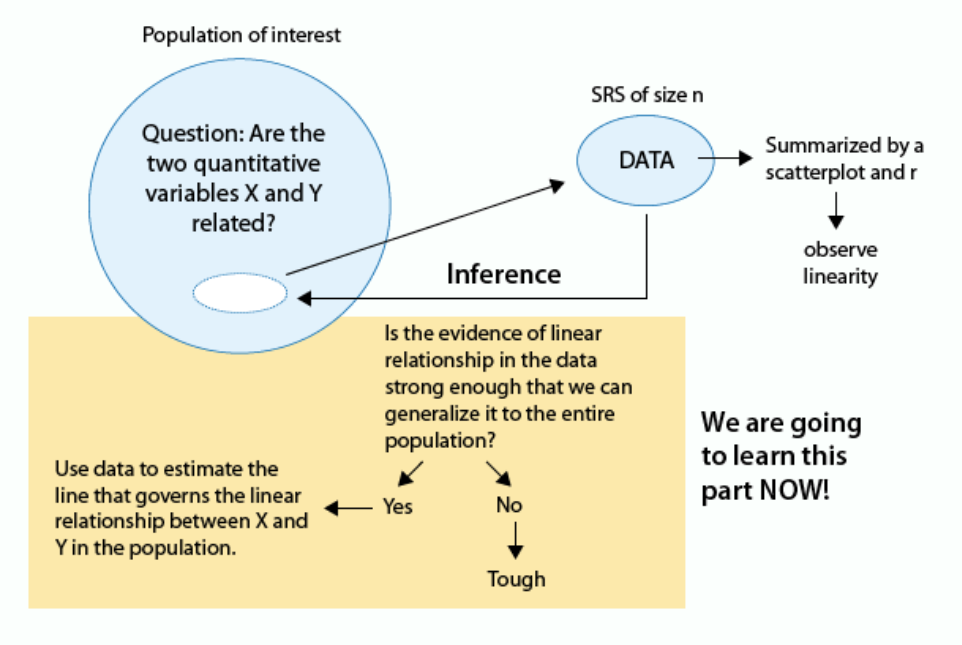
\includegraphics[width=.6\textwidth]{inferqq1.png}
\end{figure}
Finding the least squares regression line actually belongs to the inference unit, and while it is true that it is the line that best fits (in some sense) the observed data, it is really an estimate of the true linear relationship that exists in the population. \par
\begin{enumerate}
\item Making hypothesis
    $H_0$: There is no linear relationship between X and Y.
    $H_a$: There is a linear relationship between X and Y.
\item Hypothesis testing (t-test) and the conditions to perform the test.
\begin{itemize}
\item the observed data indeed look linear (otherwise it would not make sense to try and generalize them)
\item the observations are independent
\item there are no extreme outliers in the data
\item the sample size is fairly large
\end{itemize}
\item Find a test statistic value and p-value.\\
The test assesses the strength of evidence provided by the data (as seen in the scatterplot and measured by the correlation r) and reports a p-value. The p-value is the probability of getting data such as that observed assuming that, in reality, no linear relationship exists between X and Y in the population.
\item Make a conclusion.\\
Based on the p-value, we draw our conclusions. A small p-value will indicate that we reject $H_0$ and conclude that the data provide enough evidence of a real linear relationship between X and Y in the population.
\end{enumerate}
%\section{Exercises}
\bibliographystyle{template}
\bibliography{/home/cao/Dropbox/ResearchBib.bib}
\end{document}
